\begin{apendicesenv}

% Imprime uma página indicando o início dos apêndices
\partapendices

% Para cada apêndice, um \chapter


% ==============================================================================
\chapter{Experiment 1 (EX1)}
% ==============================================================================

\section{F-score - EX1}

\begin{figure}[!htb]
    \centering
    % 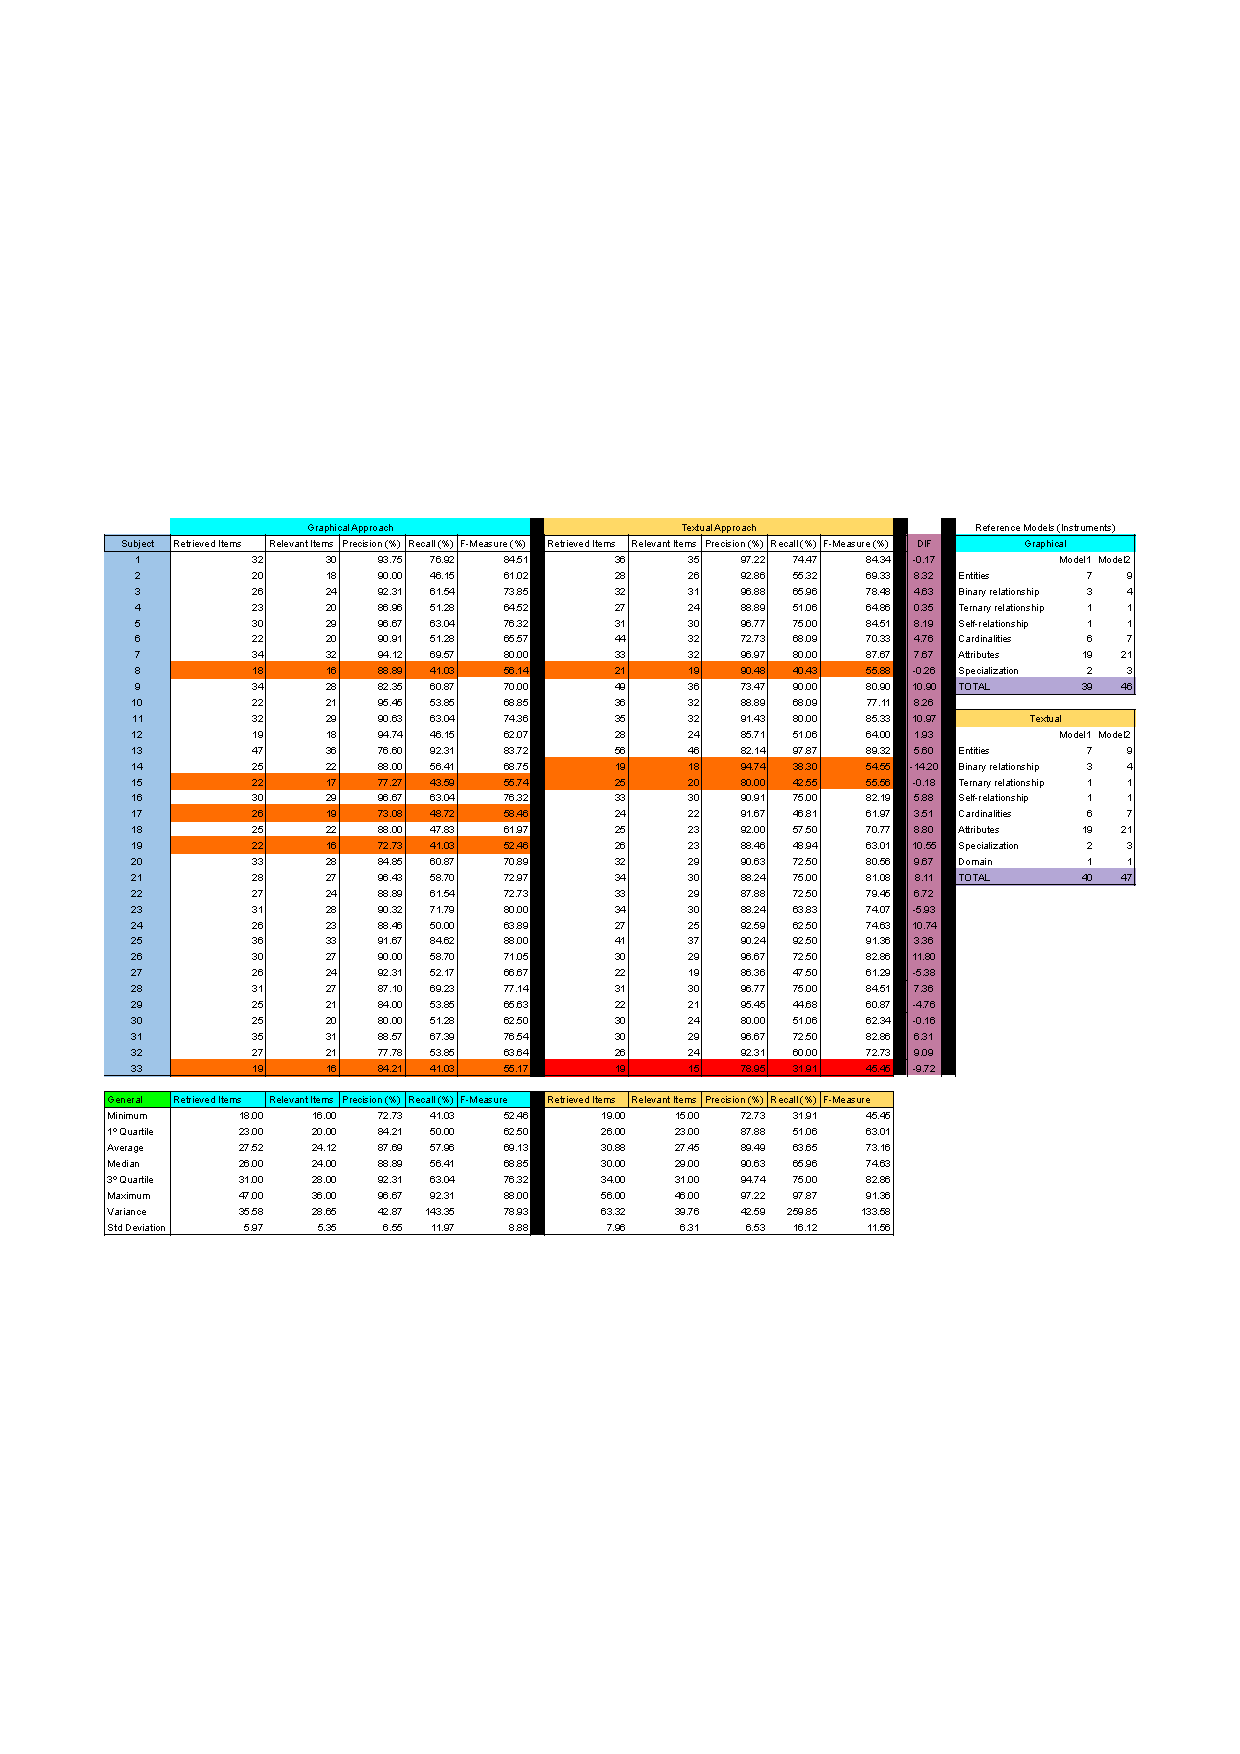
\includegraphics[]{postextuais/appendix/EX1-Results.pdf}
    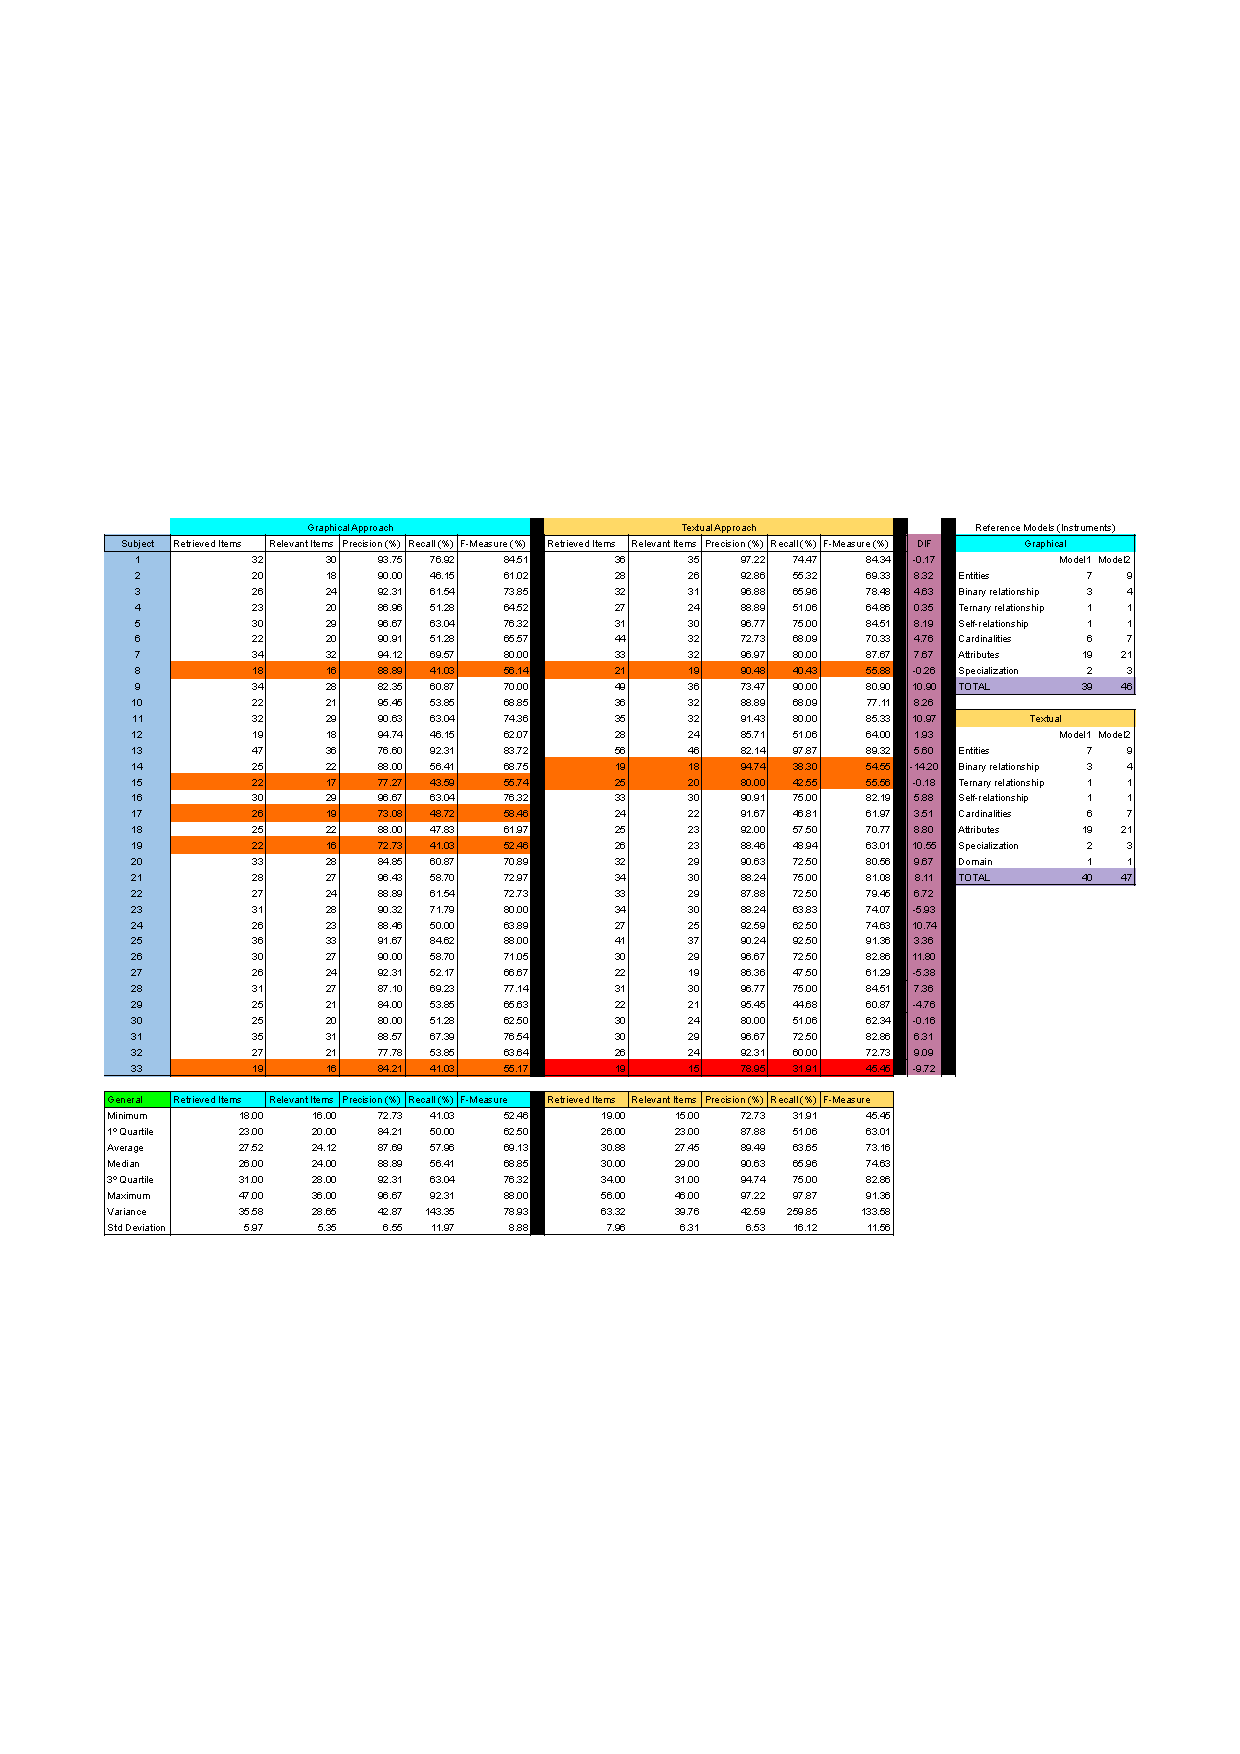
\includepdf[pages=-, frame=false, scale=0.90]{postextuais/appendix/EX1-Results.pdf}
    % \caption{EX1 - F-Score.}
    \label{fig:ex1FScore}
\end{figure}

\newpage

\section{Times - EX1}

\begin{figure}[!htb]
    \centering
    % 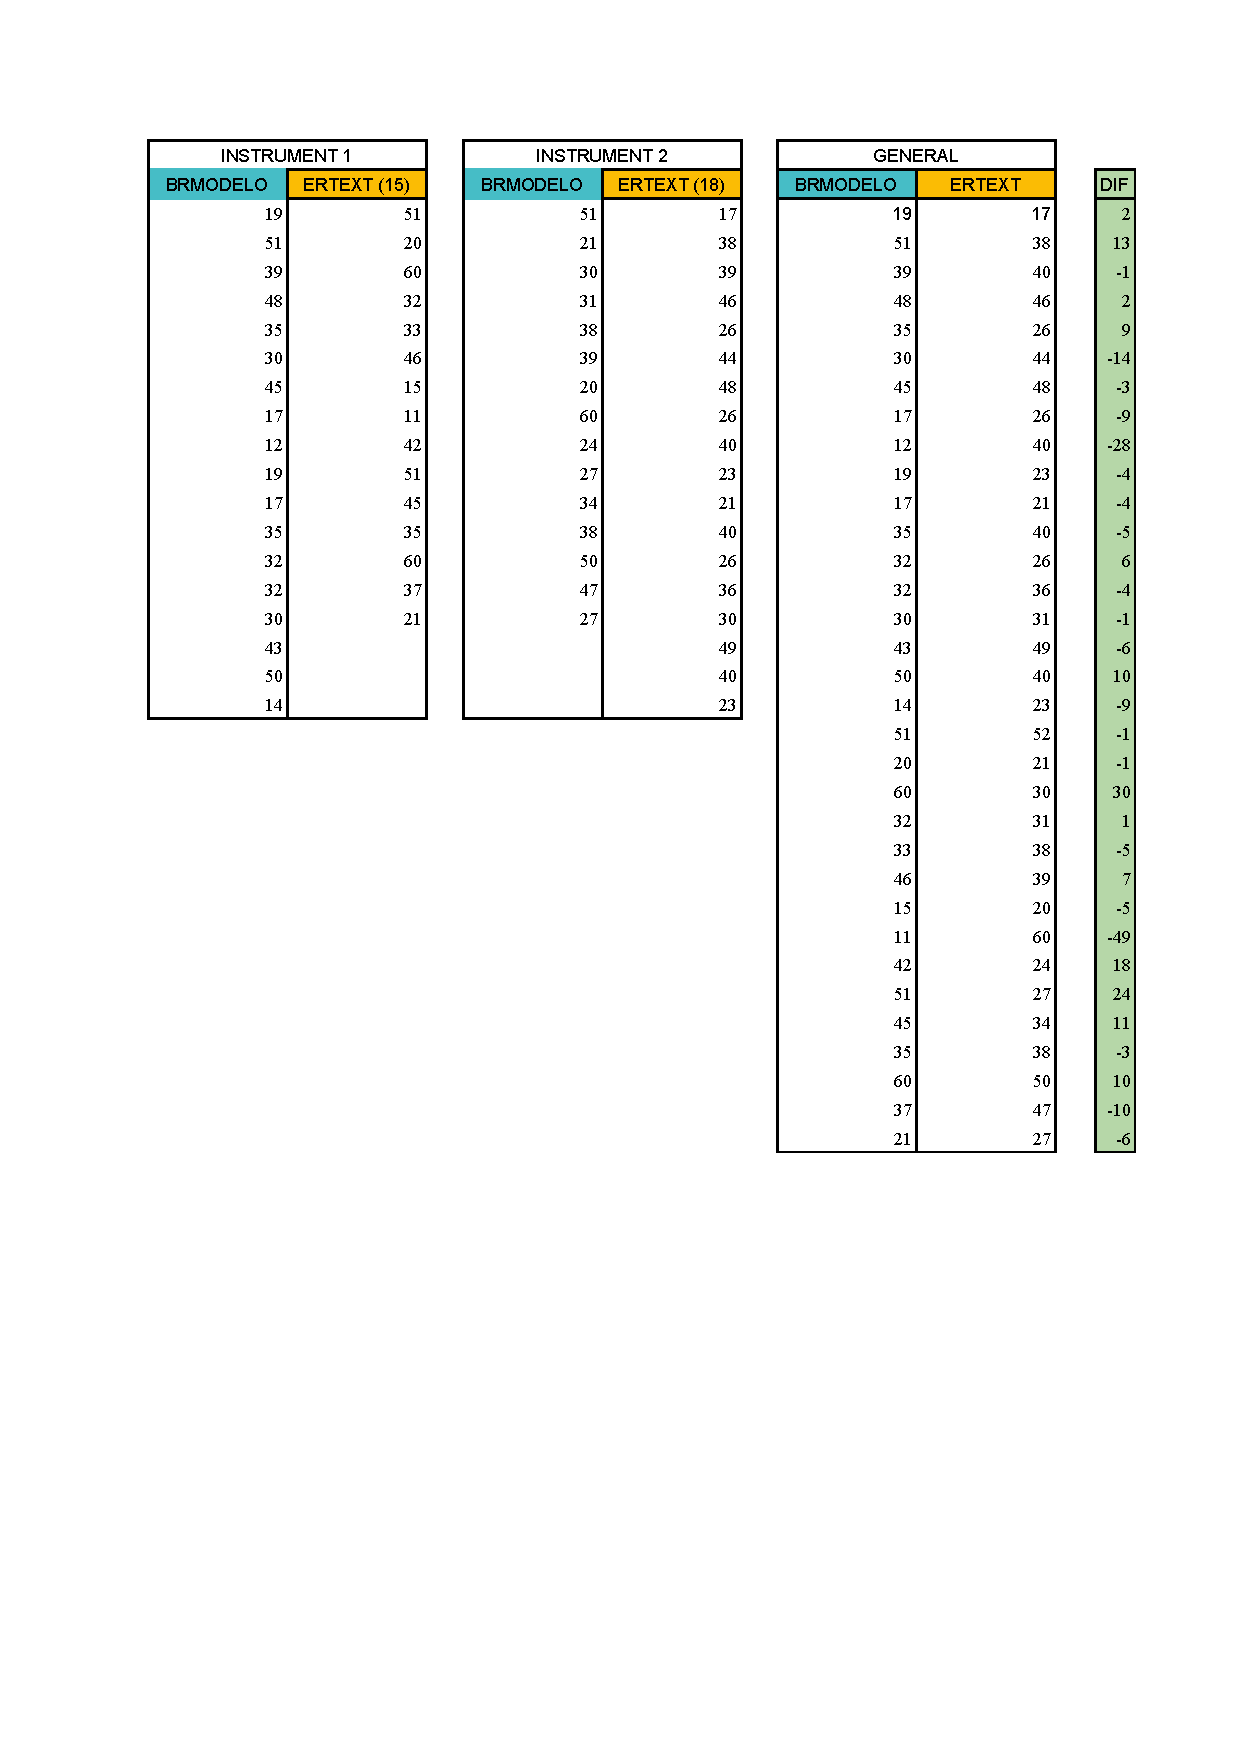
\includegraphics[]{postextuais/appendix/EX1-Results-Times.pdf}
    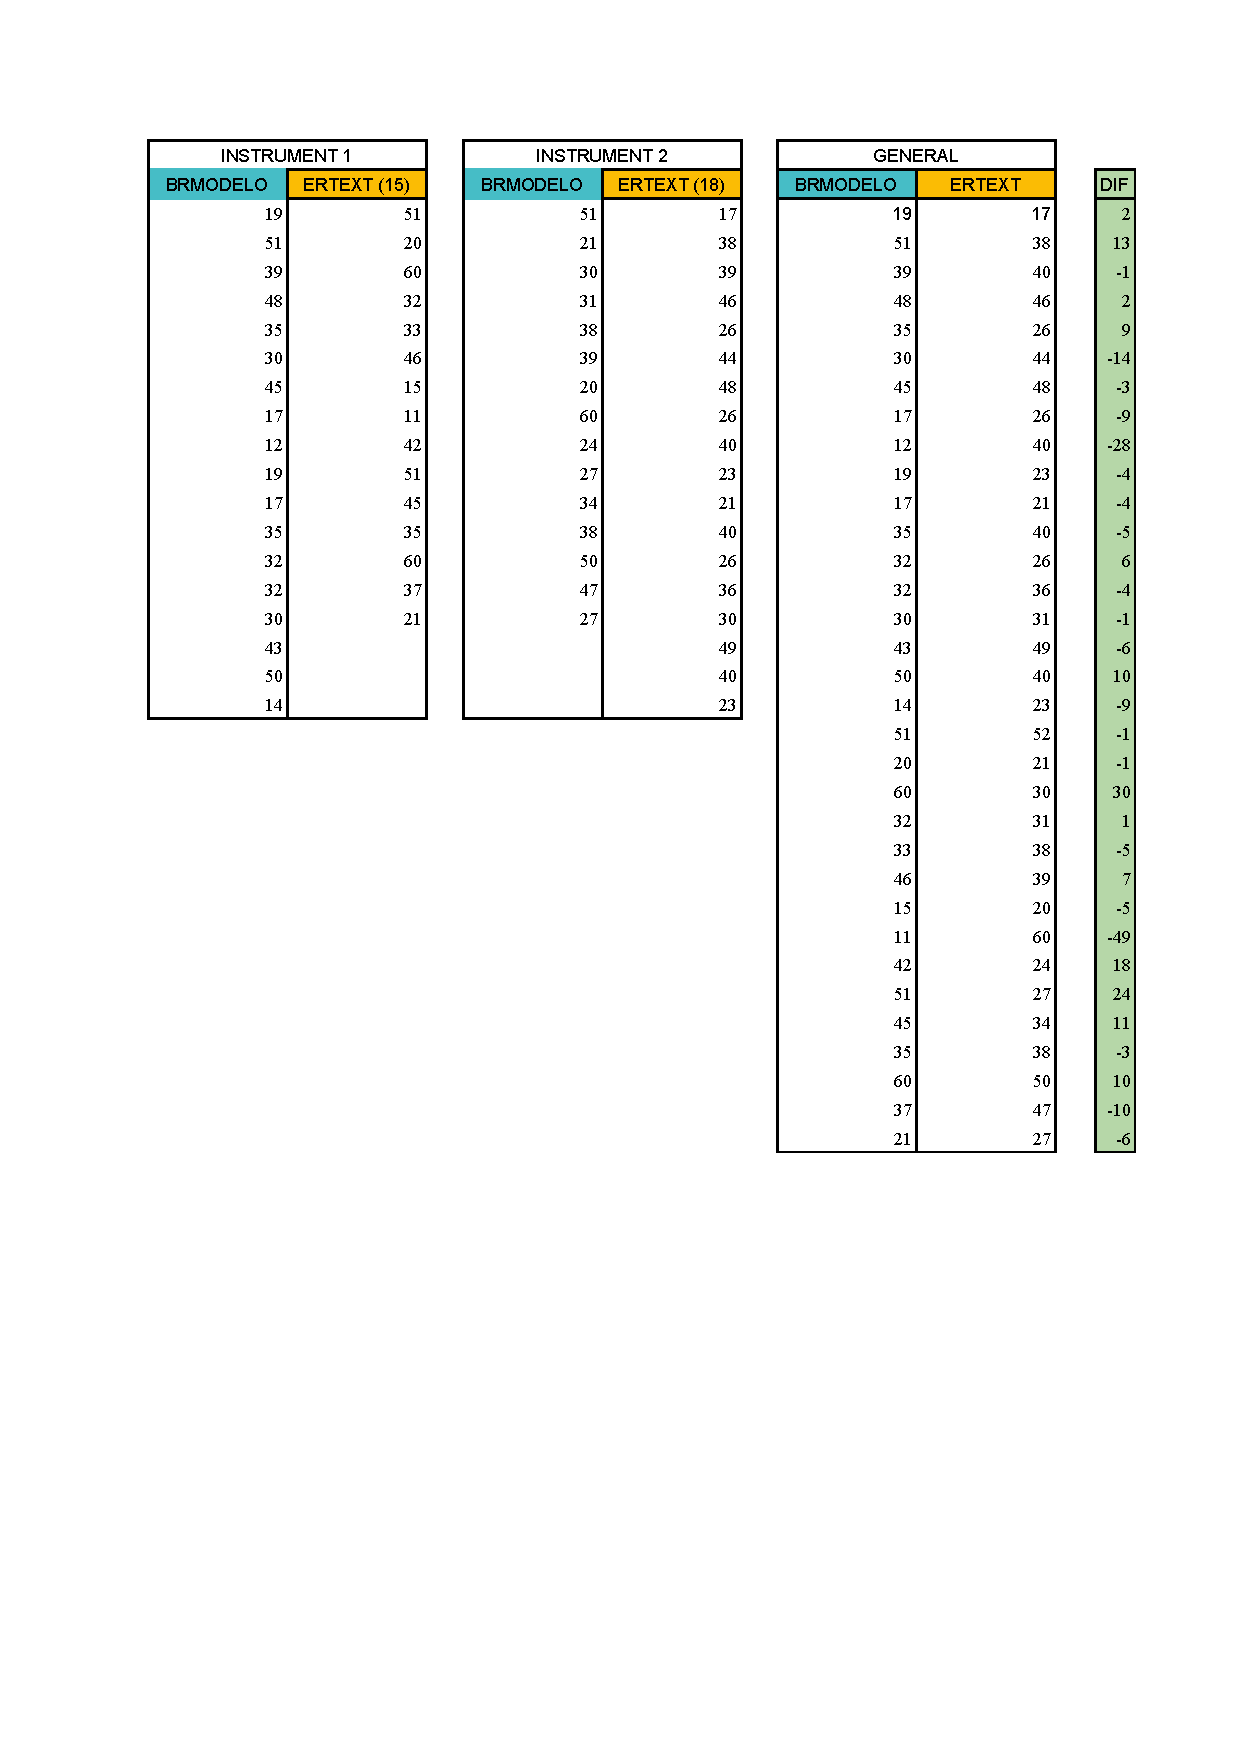
\includepdf[pages=-, frame=false, scale=0.80]{postextuais/appendix/EX1-Results-Times.pdf}
    % \caption{EX1 - times.}
    \label{fig:ex1Times}
\end{figure}

% ==============================================================================
\chapter{Experiment 2 (EX2)}
% ==============================================================================

\section{F-score - EX2}

\begin{figure}[!htb]
    \centering
    % 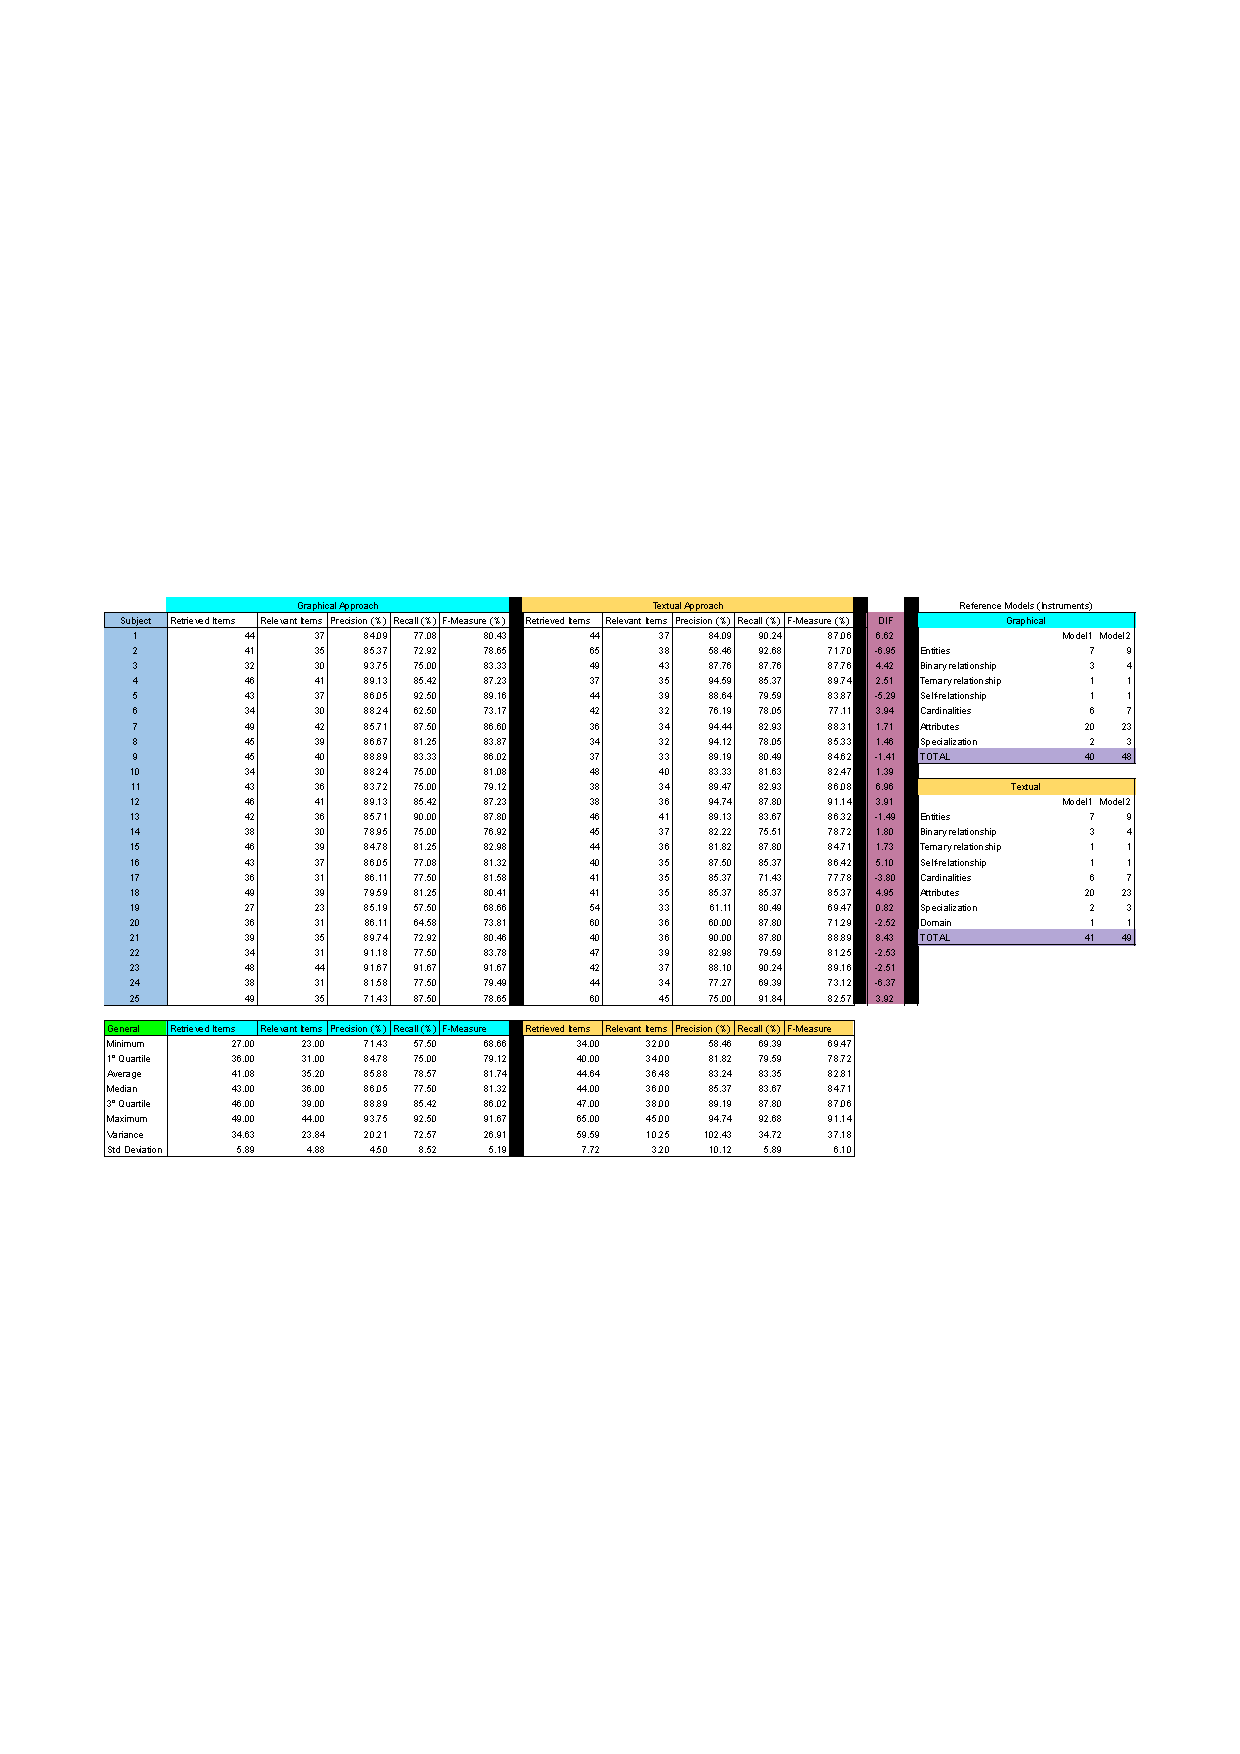
\includegraphics[]{postextuais/appendix/EX2-Results.pdf}
    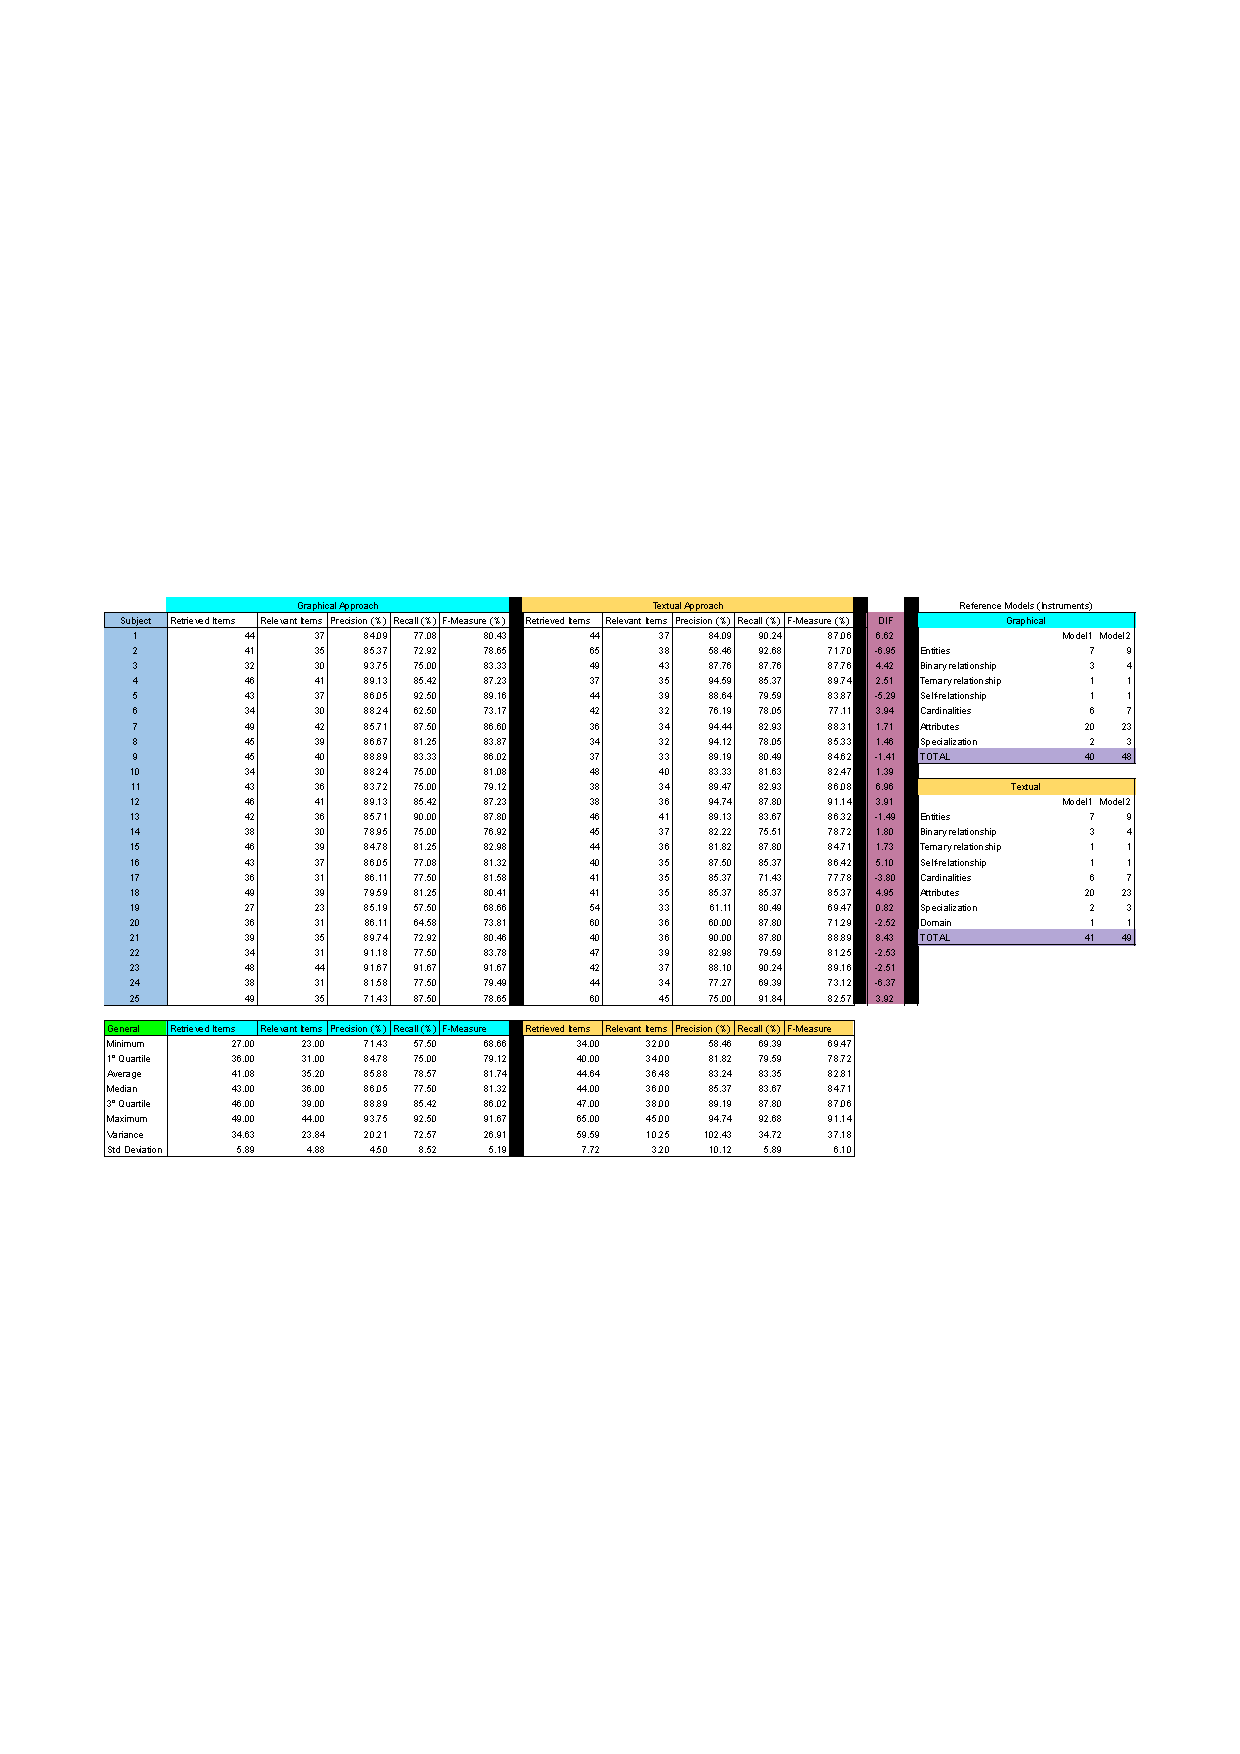
\includepdf[pages=-, frame=false, scale=0.90]{postextuais/appendix/EX2-Results.pdf}
    % \caption{EX2 - F-Score.}
    \label{fig:ex2FScore}
\end{figure}

\newpage

\section{Times - EX2}

\begin{figure}[!htb]
    \centering
    % 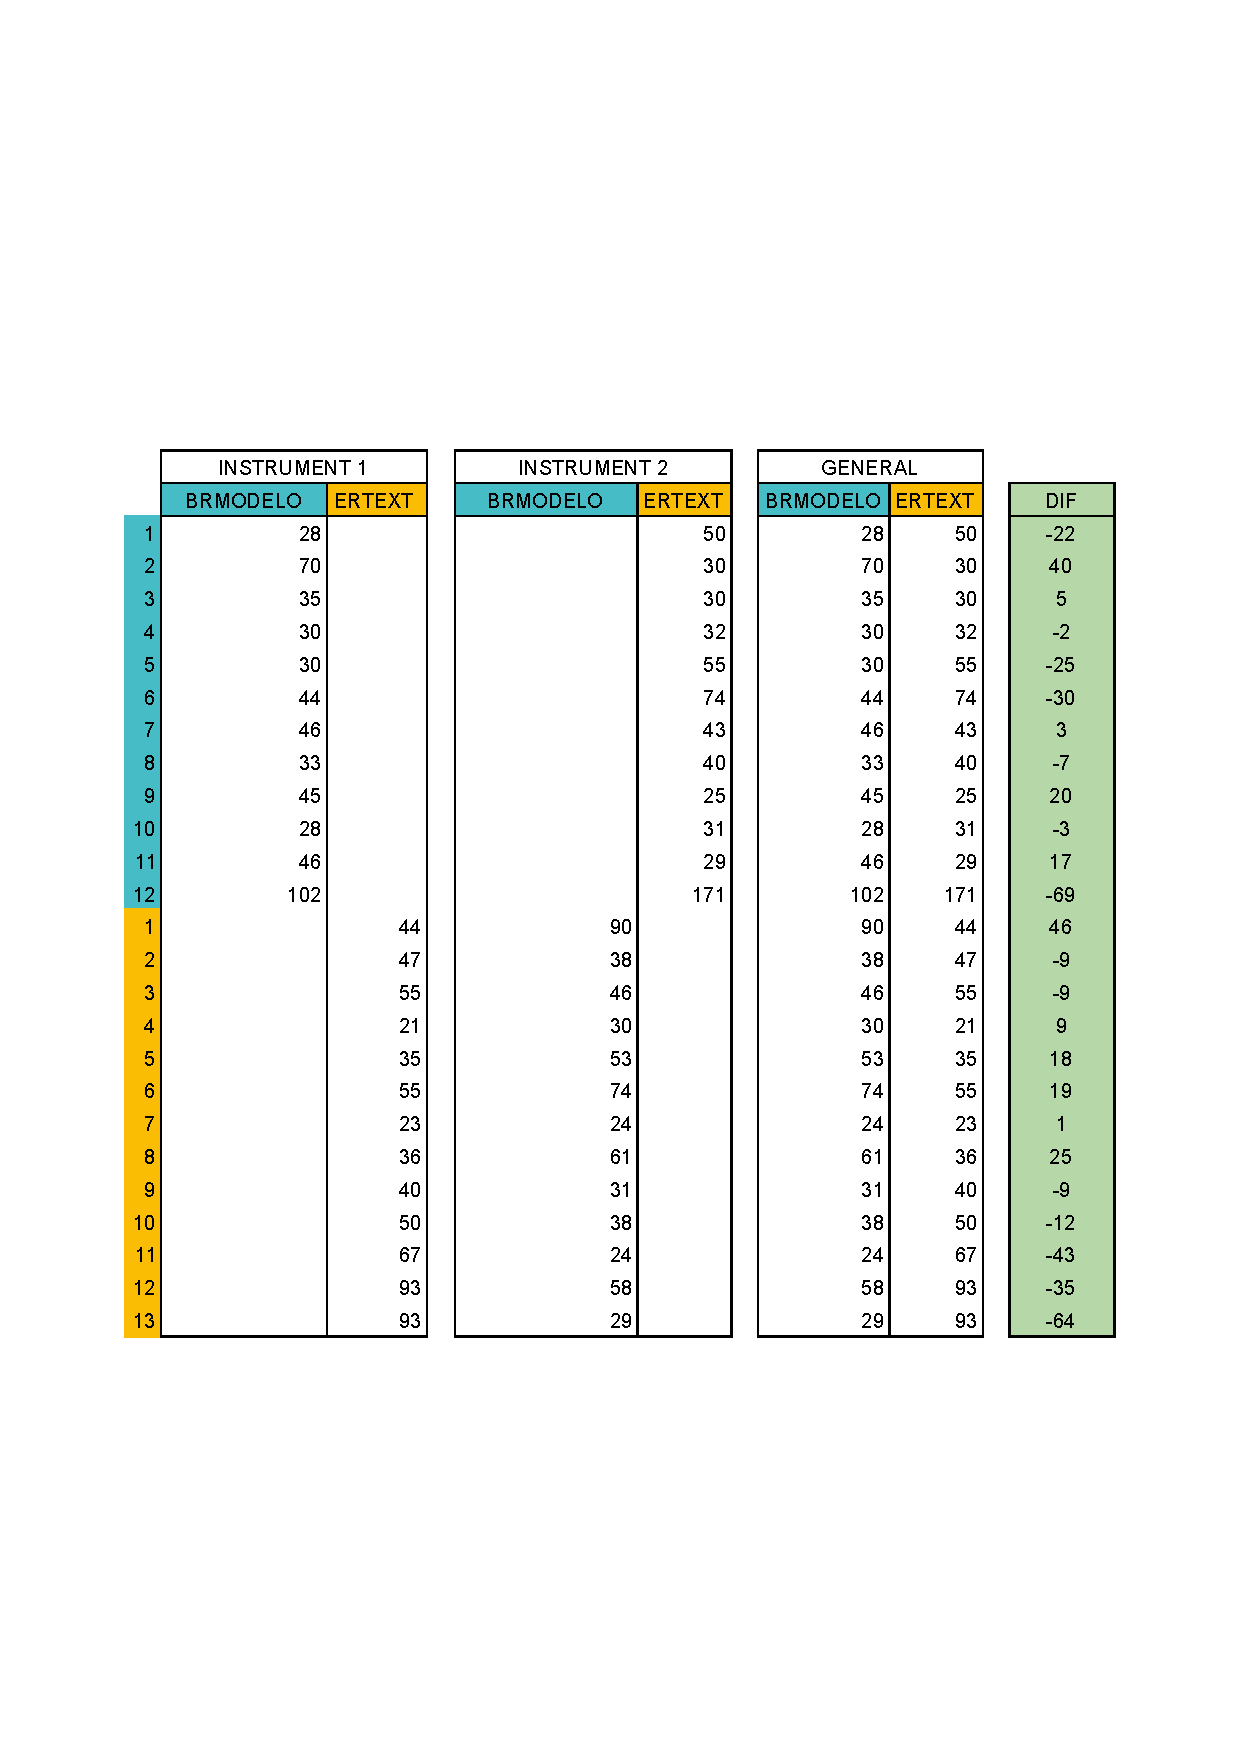
\includegraphics[]{postextuais/appendix/EX2-Results-Times.pdf}
    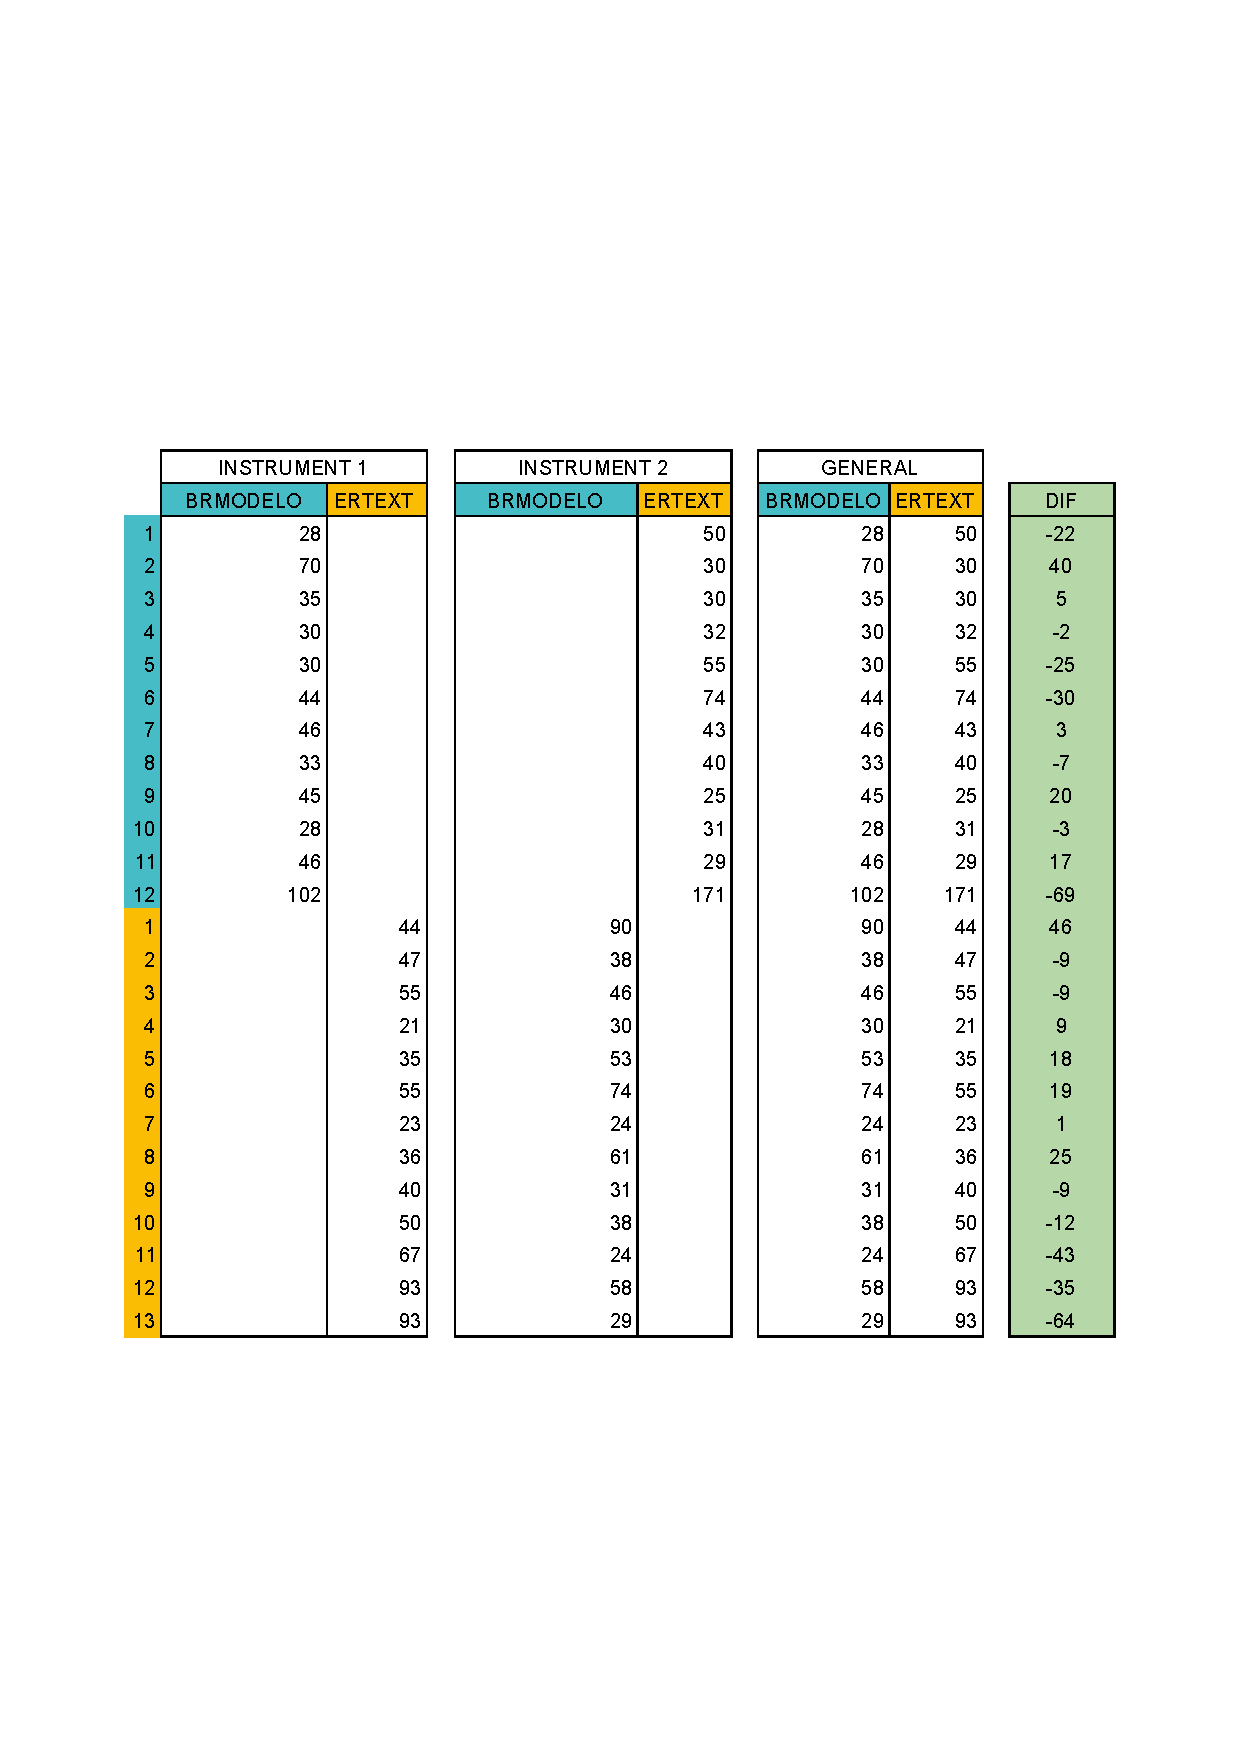
\includepdf[pages=-, frame=false, scale=0.90]{postextuais/appendix/EX2-Results-Times.pdf}
    % \caption{EX2 - Times.}
    \label{fig:ex2Times}
\end{figure}

\newpage

\section{Emocards - EX2}

\begin{figure}[!htb]
    \centering
    % 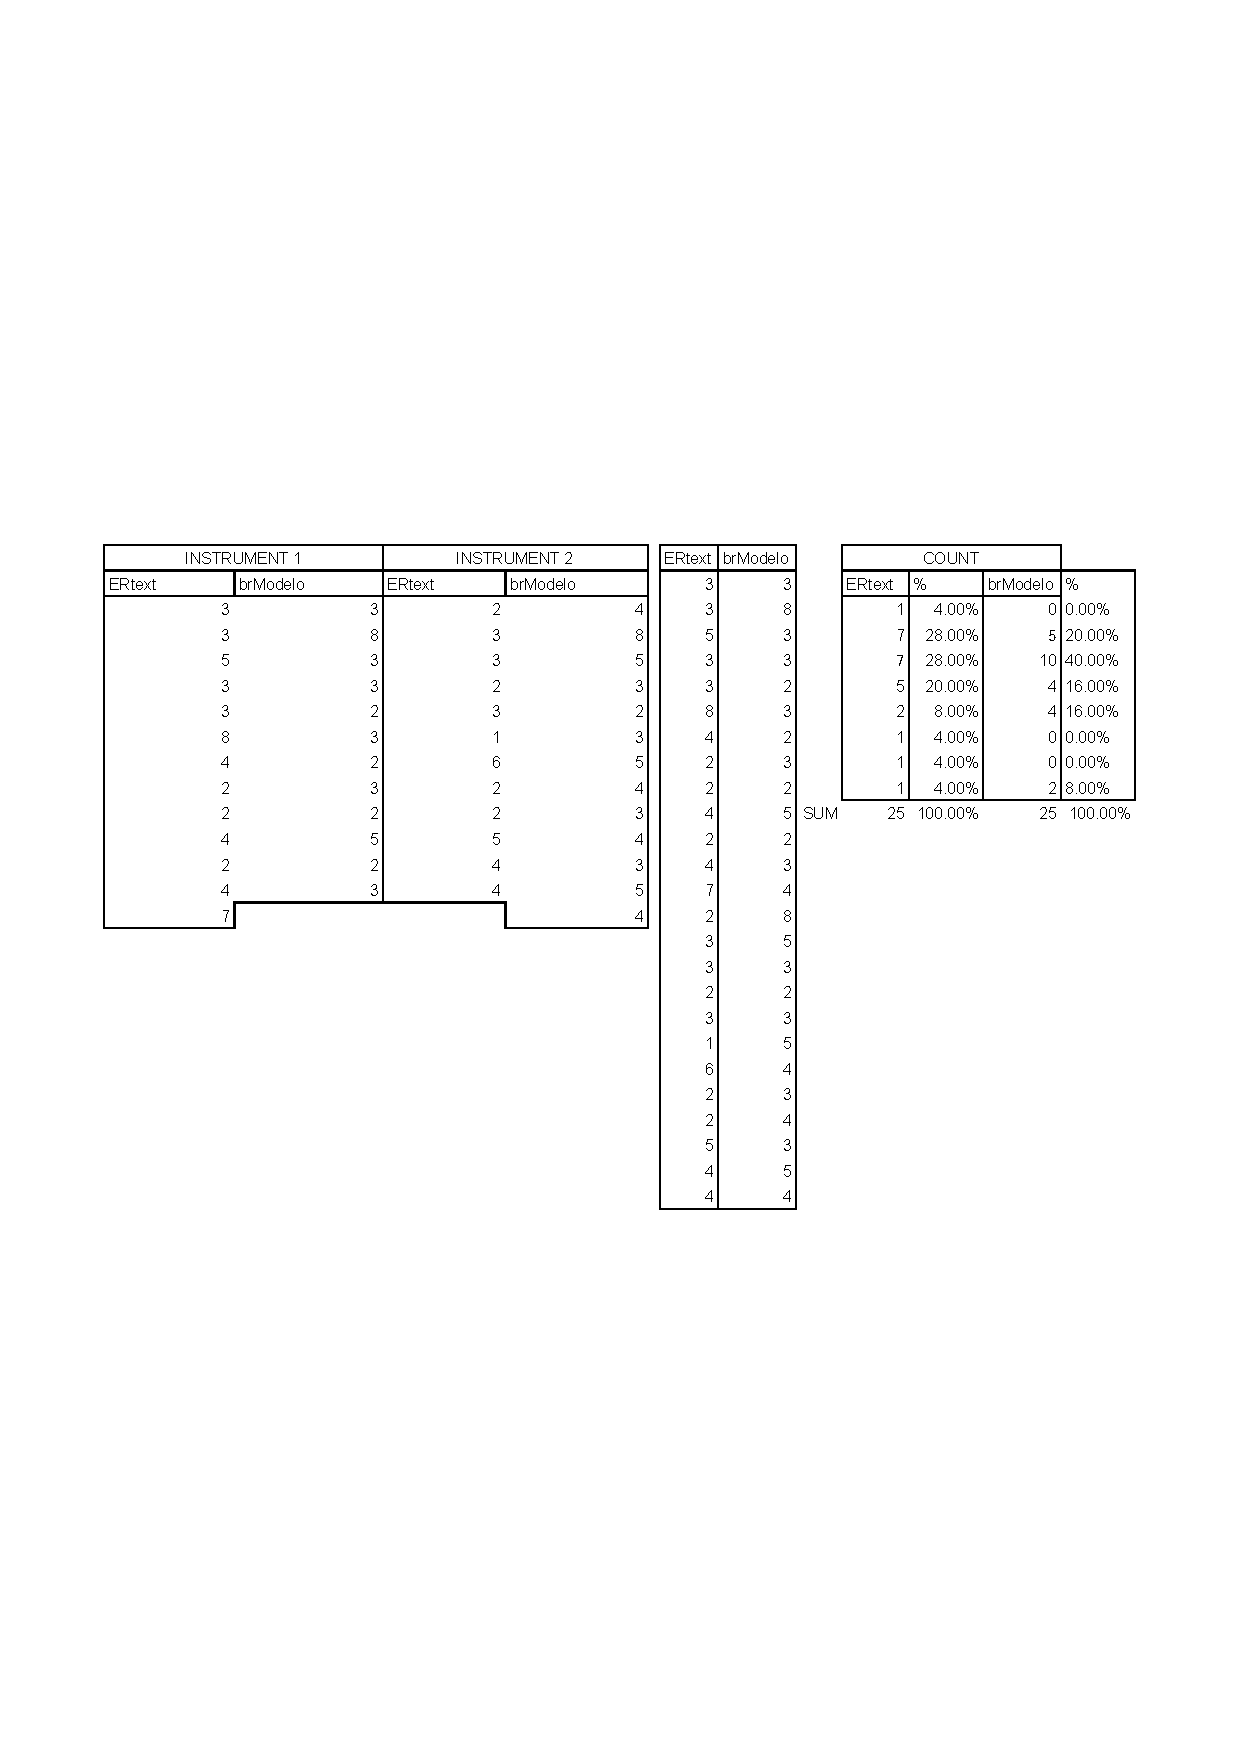
\includegraphics[]{postextuais/appendix/EX2-Results-Emocards.pdf}
    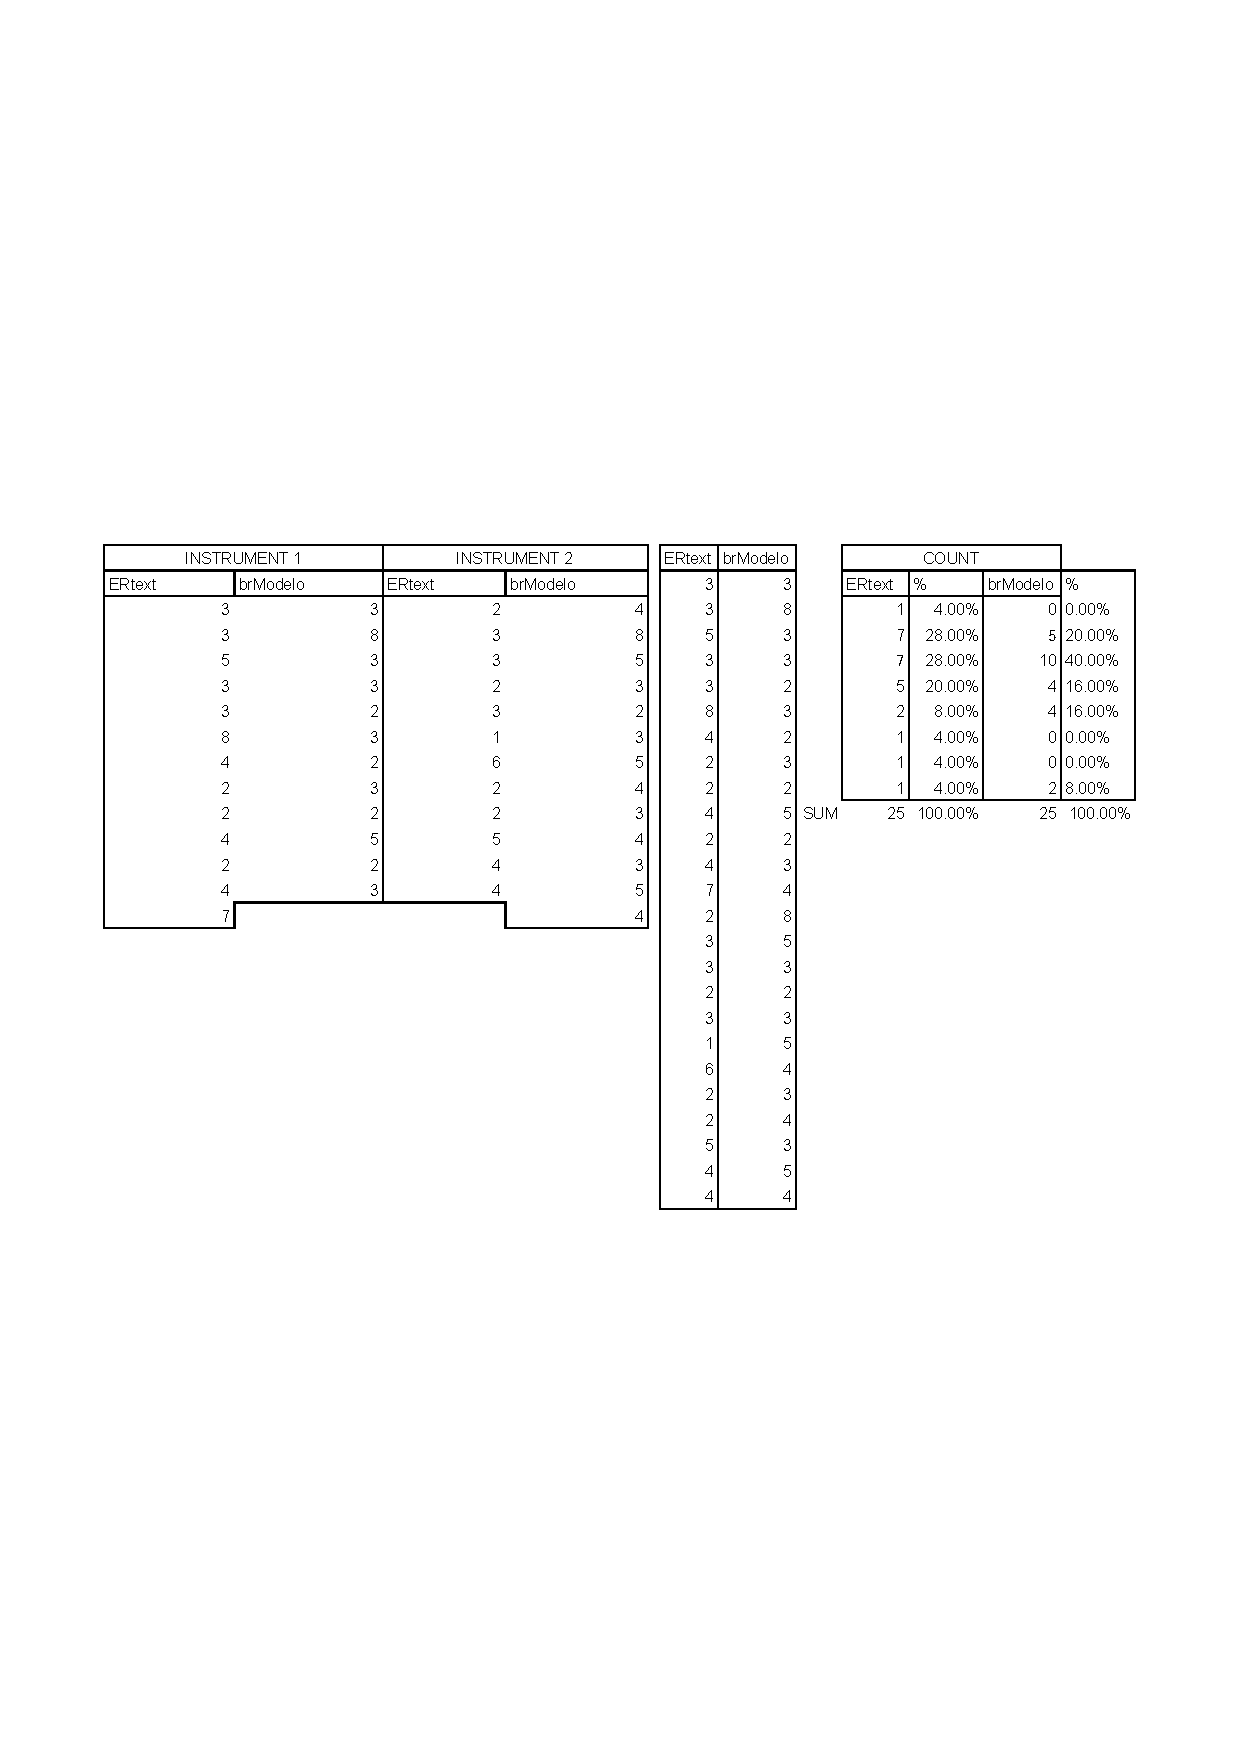
\includepdf[pages=-, frame=false, scale=0.90]{postextuais/appendix/EX2-Results-Emocards.pdf}
    % \caption{EX2 - Emocards.}
    \label{fig:ex2Emocards}
\end{figure}



% ==============================================================================
\chapter{Experiment 3 (EX3)}
% ==============================================================================

\section{Emocards - brModelo - EX3}

\begin{figure}[!htb]
    \centering
    % 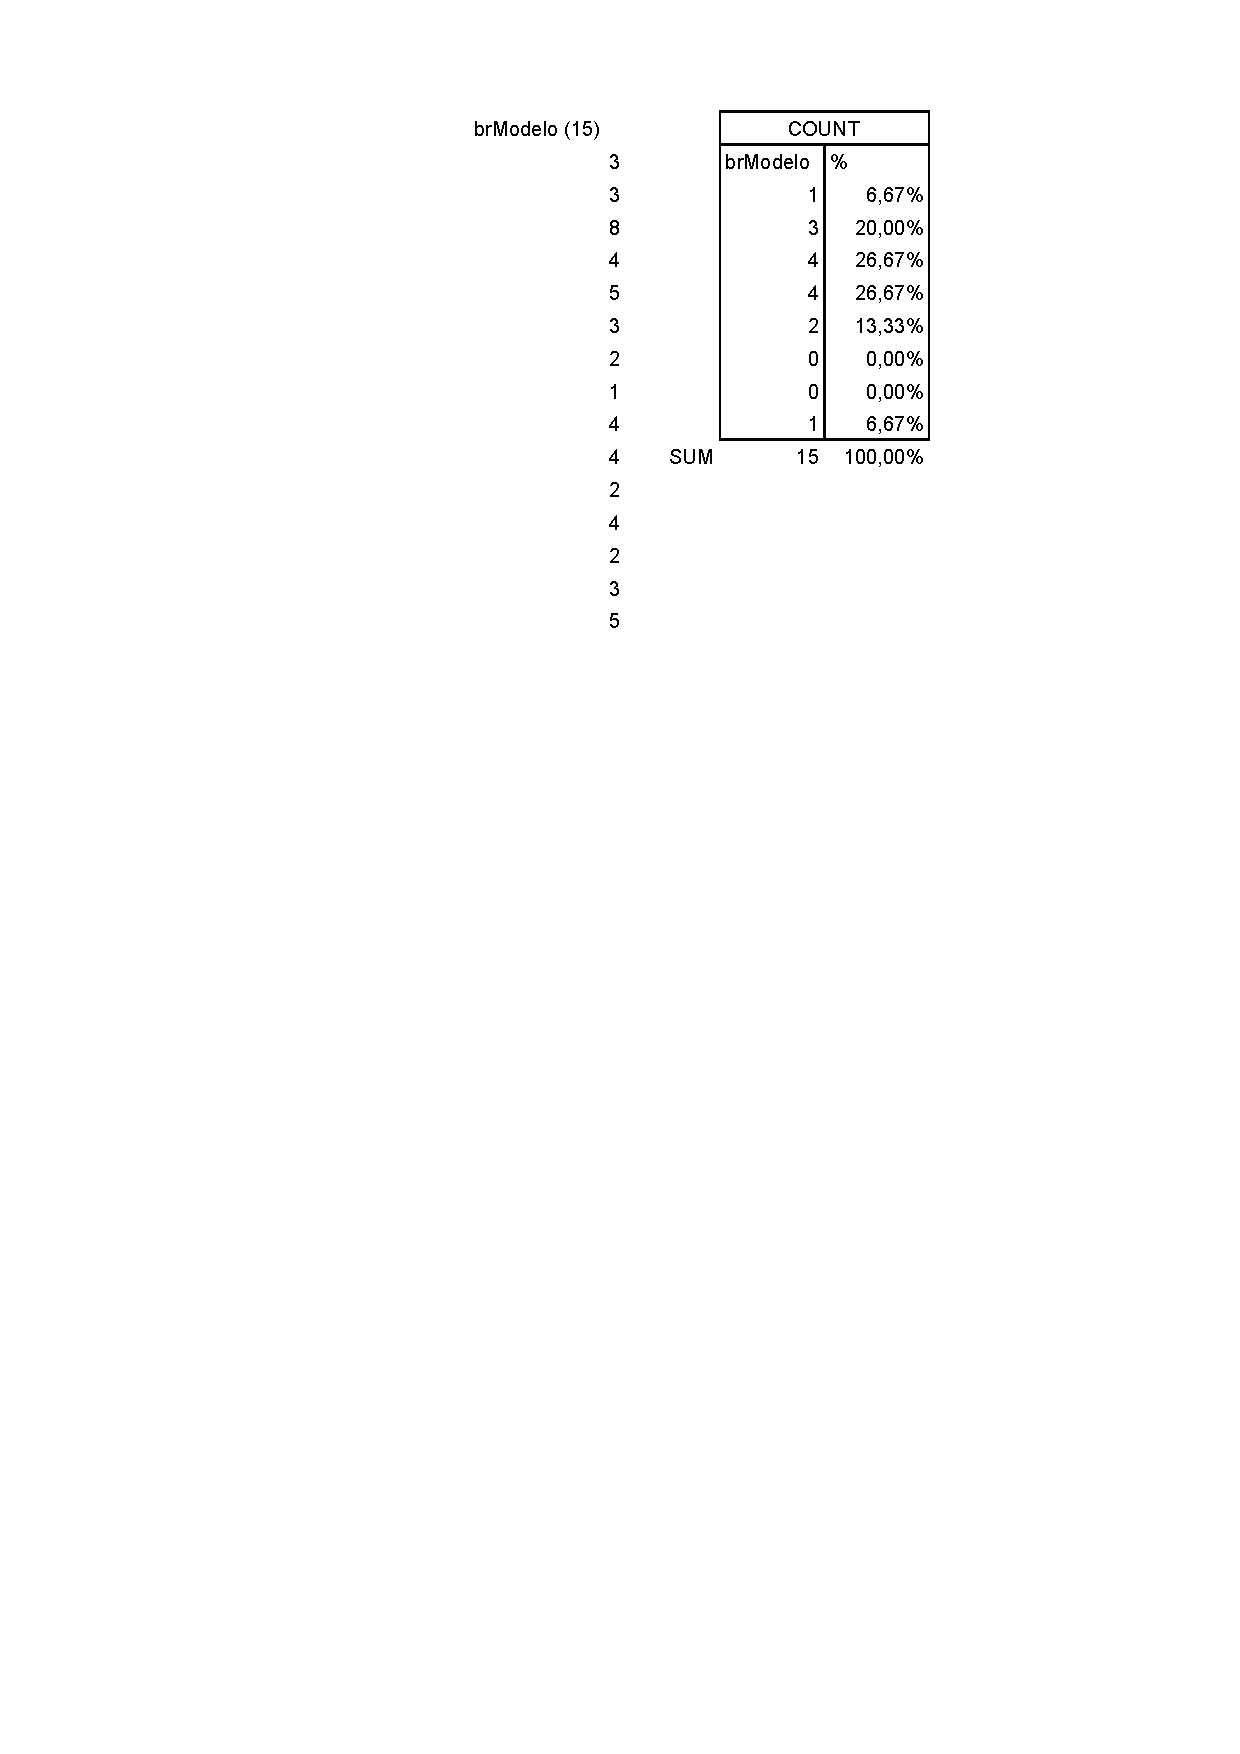
\includegraphics[]{postextuais/appendix/EX3- Emocards-brModelo.pdf}
    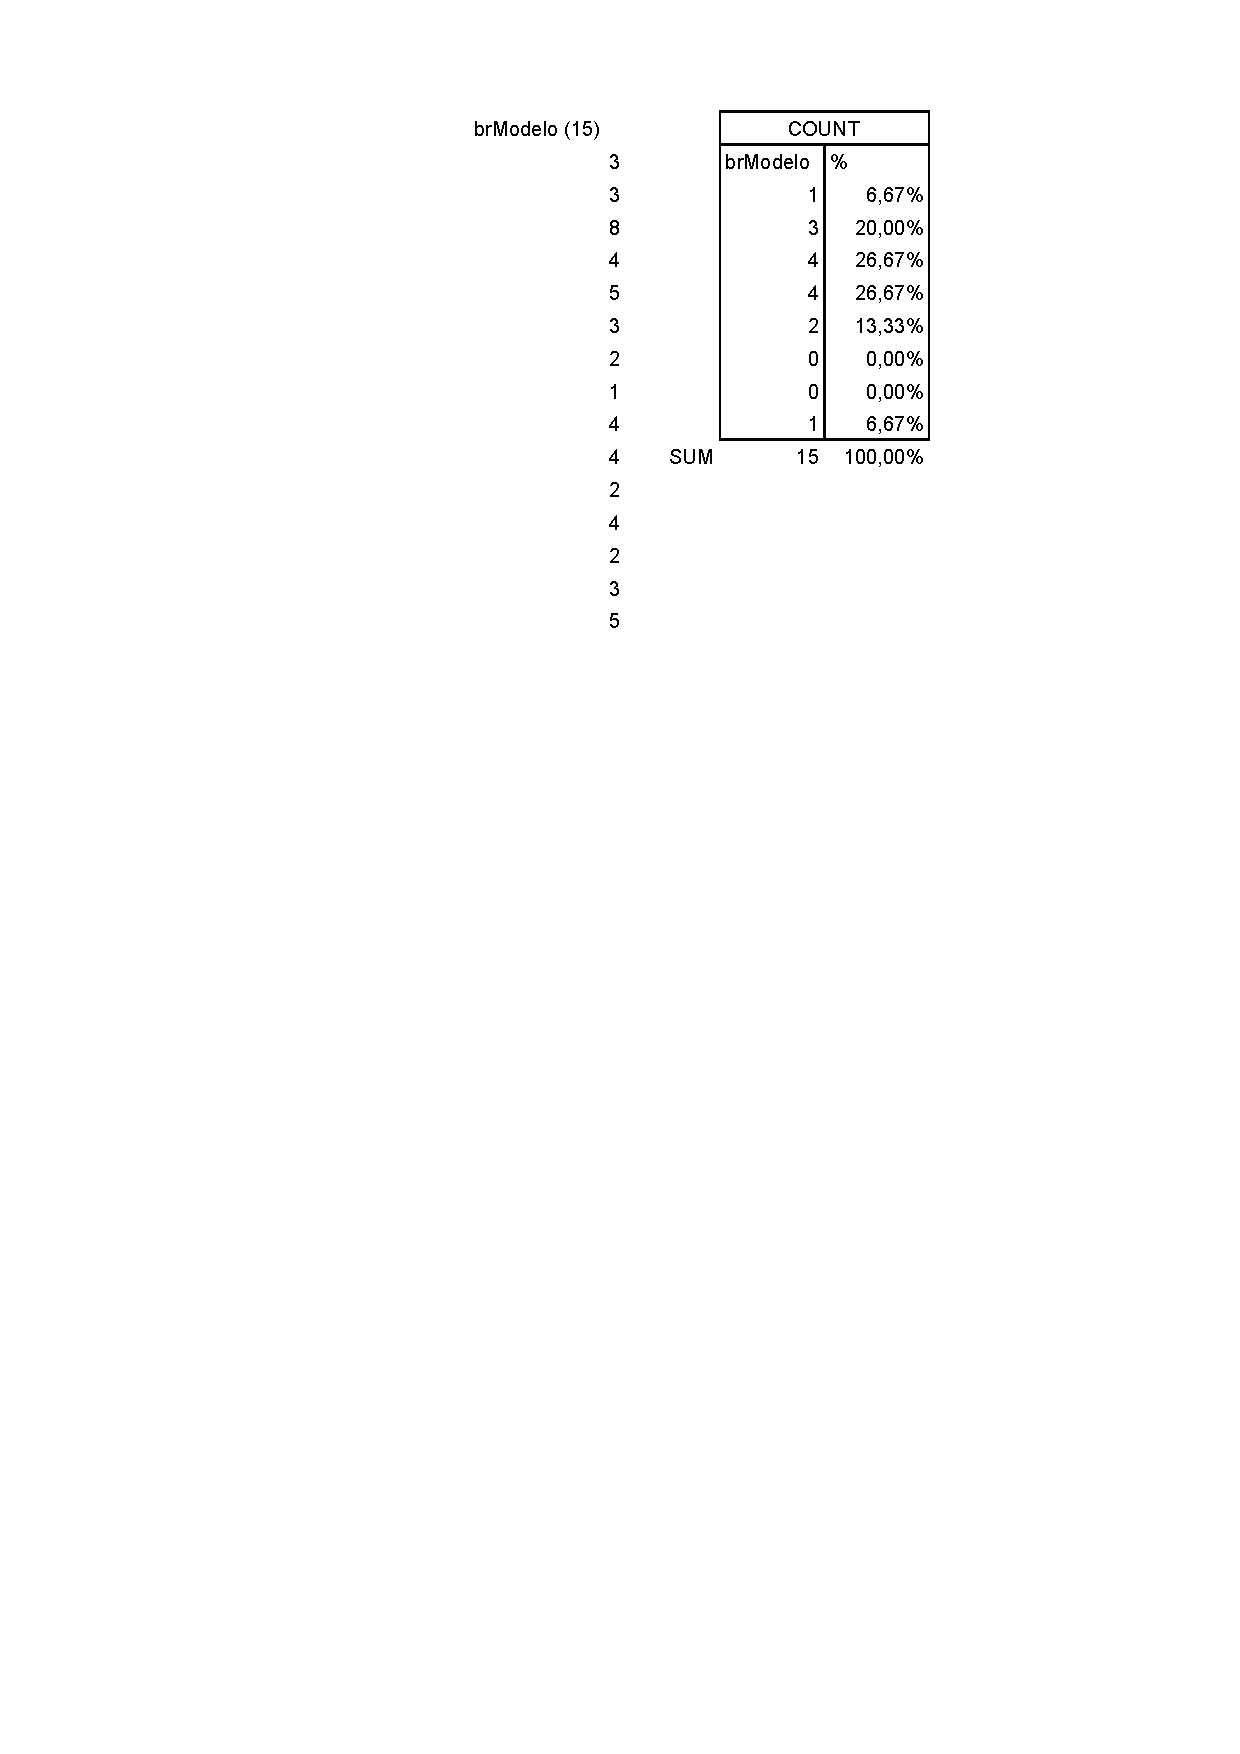
\includepdf[pages=-, frame=false, scale=0.70]{postextuais/appendix/EX3- Emocards-brModelo.pdf}
    % \caption{EX3 - Emocards - brModelo.}
    \label{fig:ex3EmocardsbrModelo}
\end{figure}

\newpage

\section{Emocards - ERtext - EX3}


\begin{figure}[!htb]
    \centering
    % 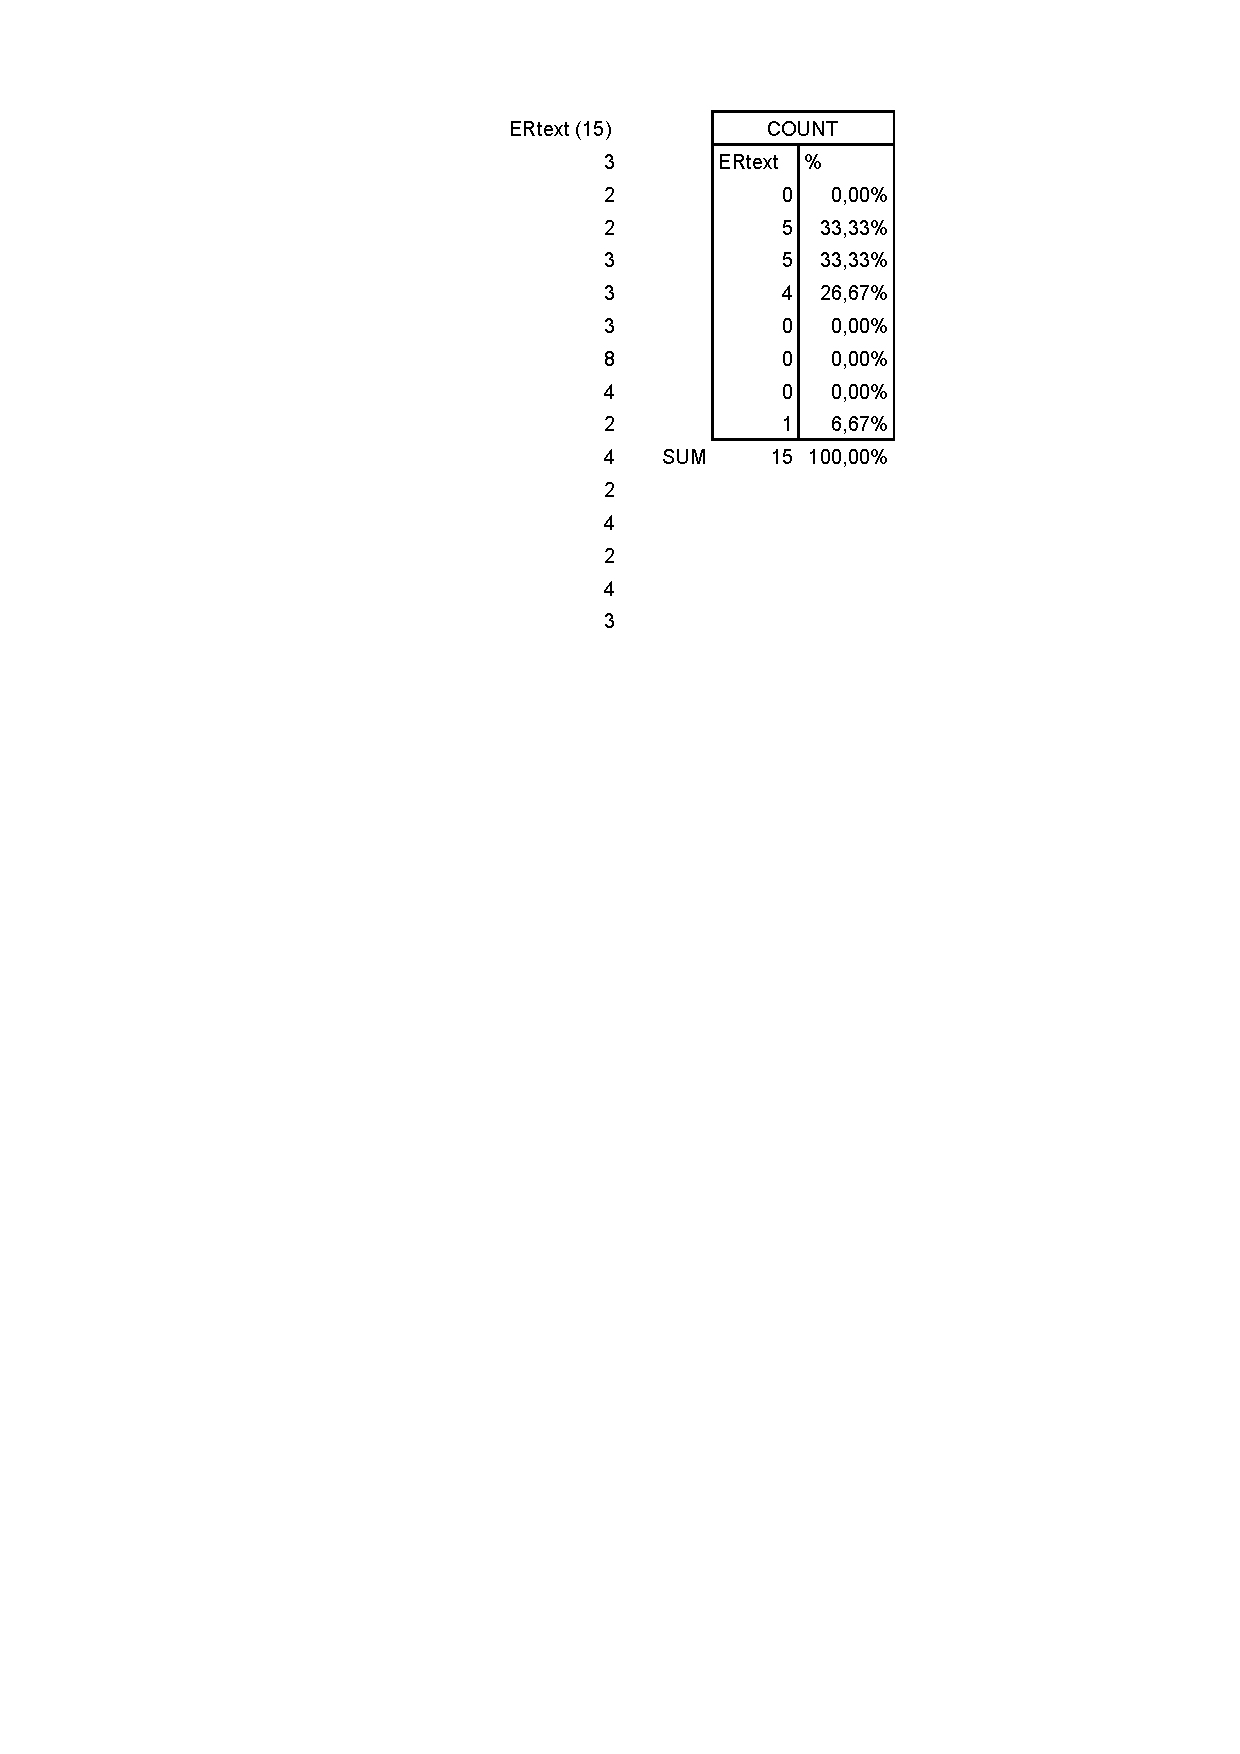
\includegraphics[]{postextuais/appendix/EX3- Emocards-ERtext.pdf}
    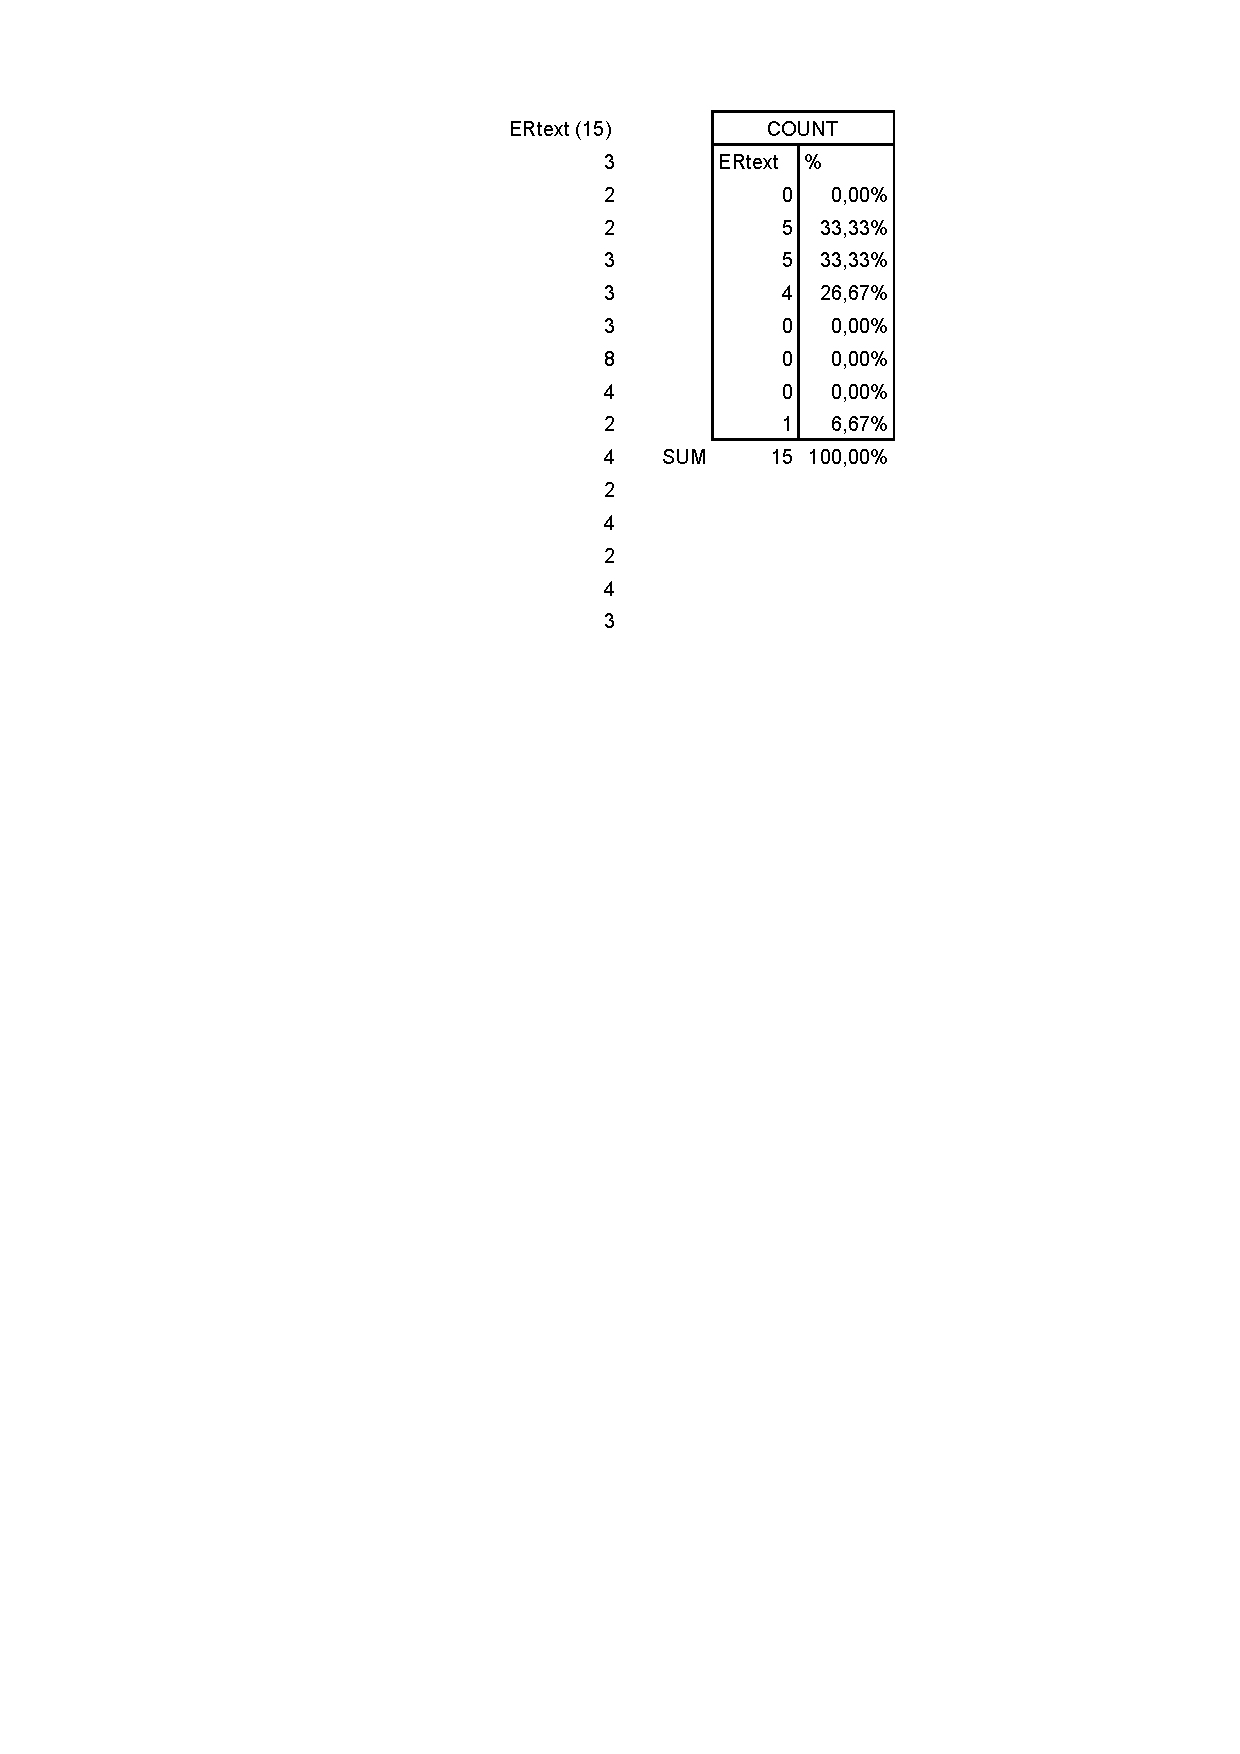
\includepdf[pages=-, frame=false, scale=0.70]{postextuais/appendix/EX3- Emocards-ERtext.pdf}
    % \caption{EX3 - Emocards - ERtext.}
    \label{fig:ex3EmocardsERtext}
\end{figure}

\newpage

\section{SUS - brModelo - EX3}

\begin{figure}[!htb]
    \centering
    % 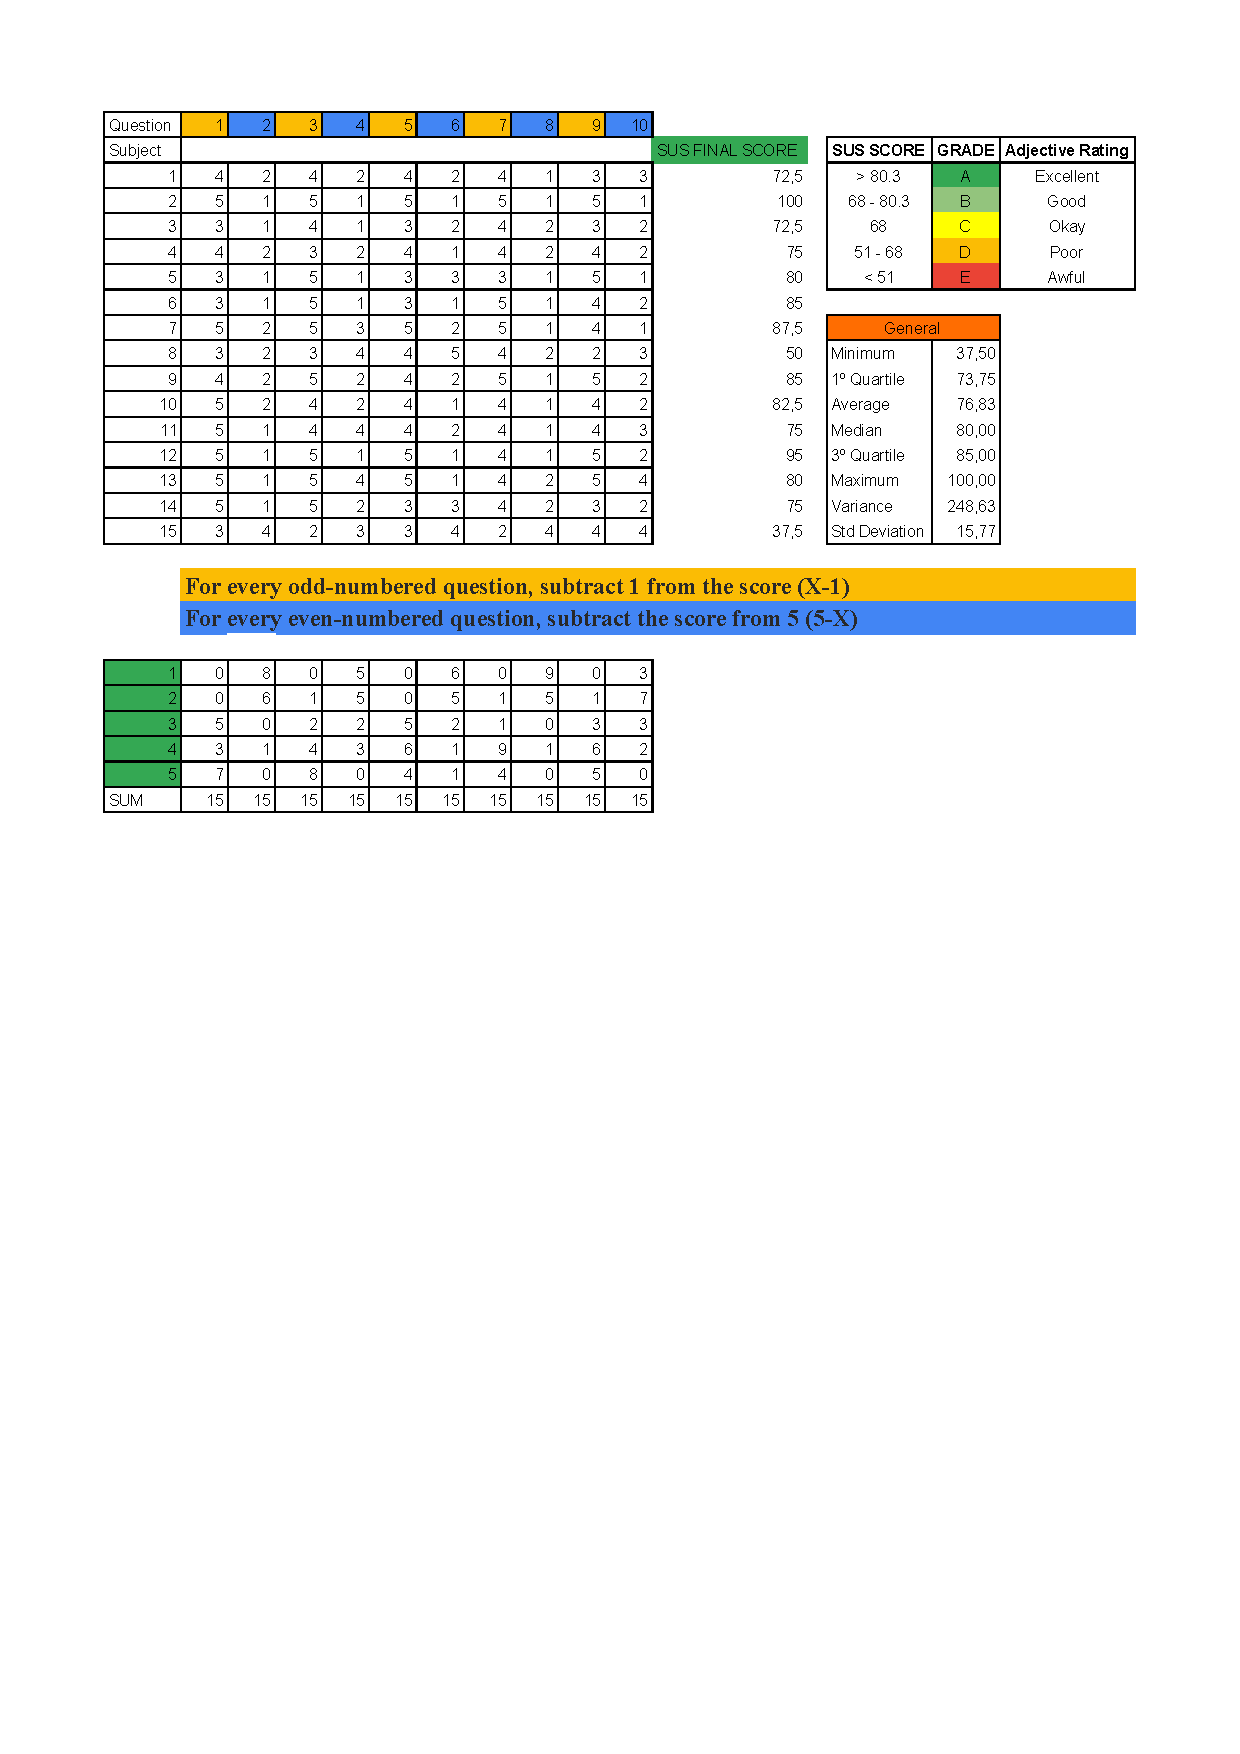
\includegraphics[]{postextuais/appendix/EX3-SUS-brModelo.pdf}
    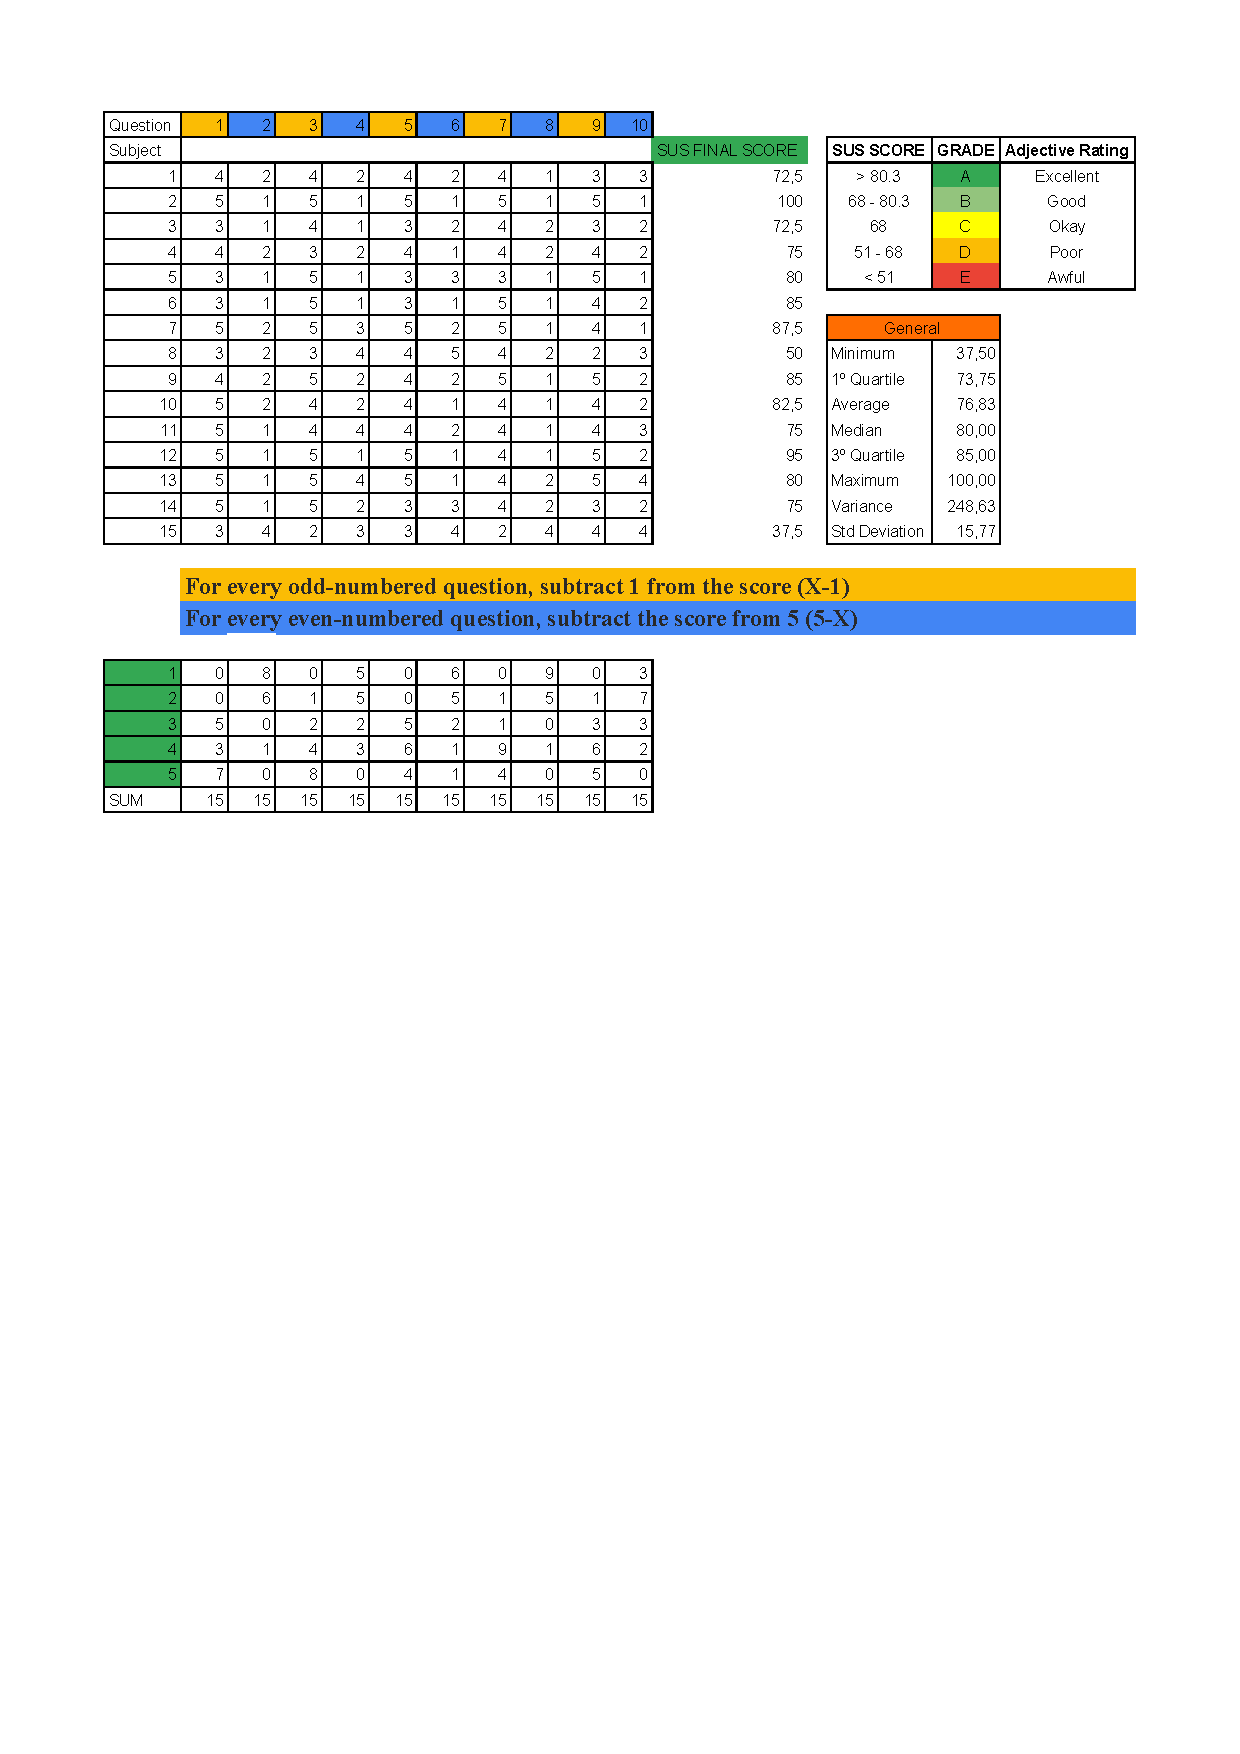
\includepdf[pages=-, frame=false, scale=0.80]{postextuais/appendix/EX3-SUS-brModelo.pdf}
    % \caption{EX3 - SUS - brModelo.}
    \label{fig:ex3EmocardsERtext}
\end{figure}

\newpage


\section{SUS - ERtext - EX3}

\begin{figure}[!htb]
    \centering
    % 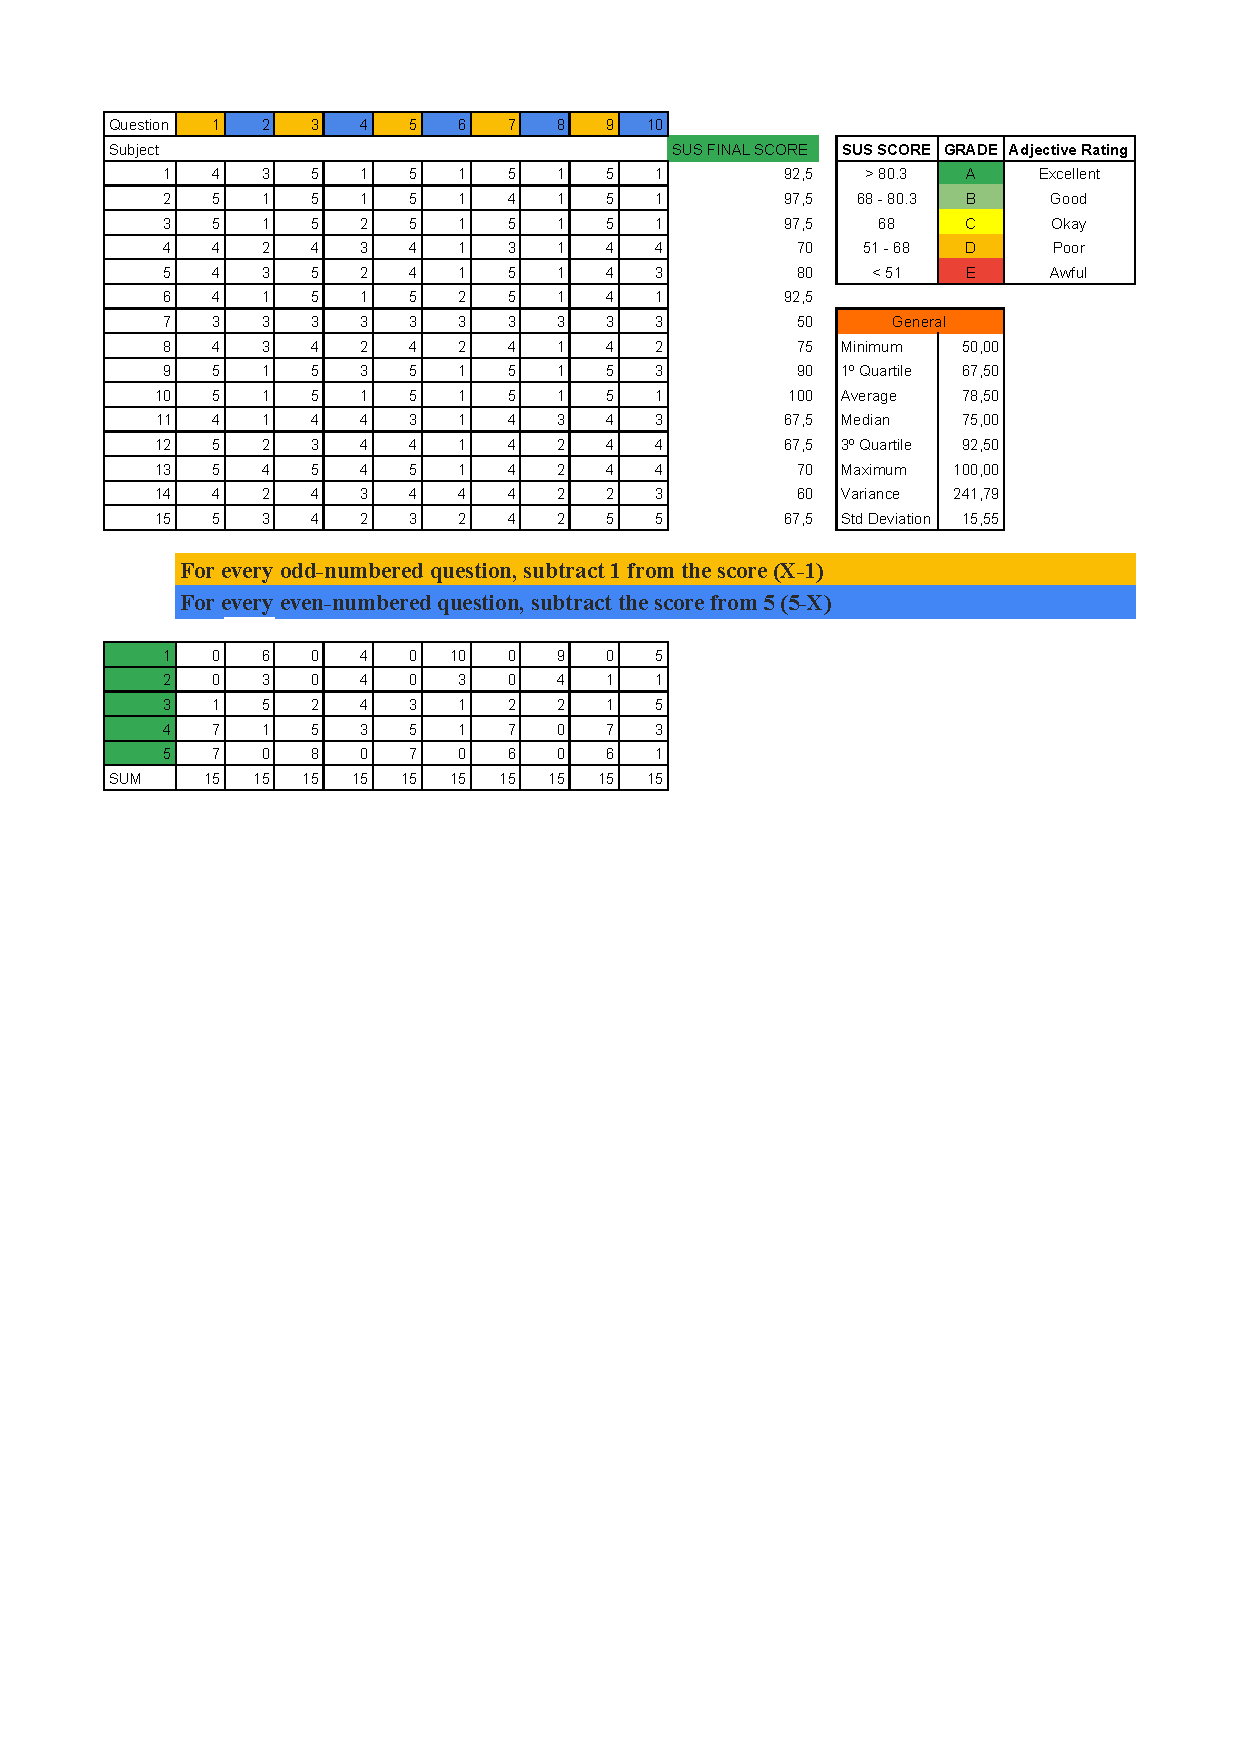
\includegraphics[]{postextuais/appendix/EX3-SUS-ERtext.pdf}
    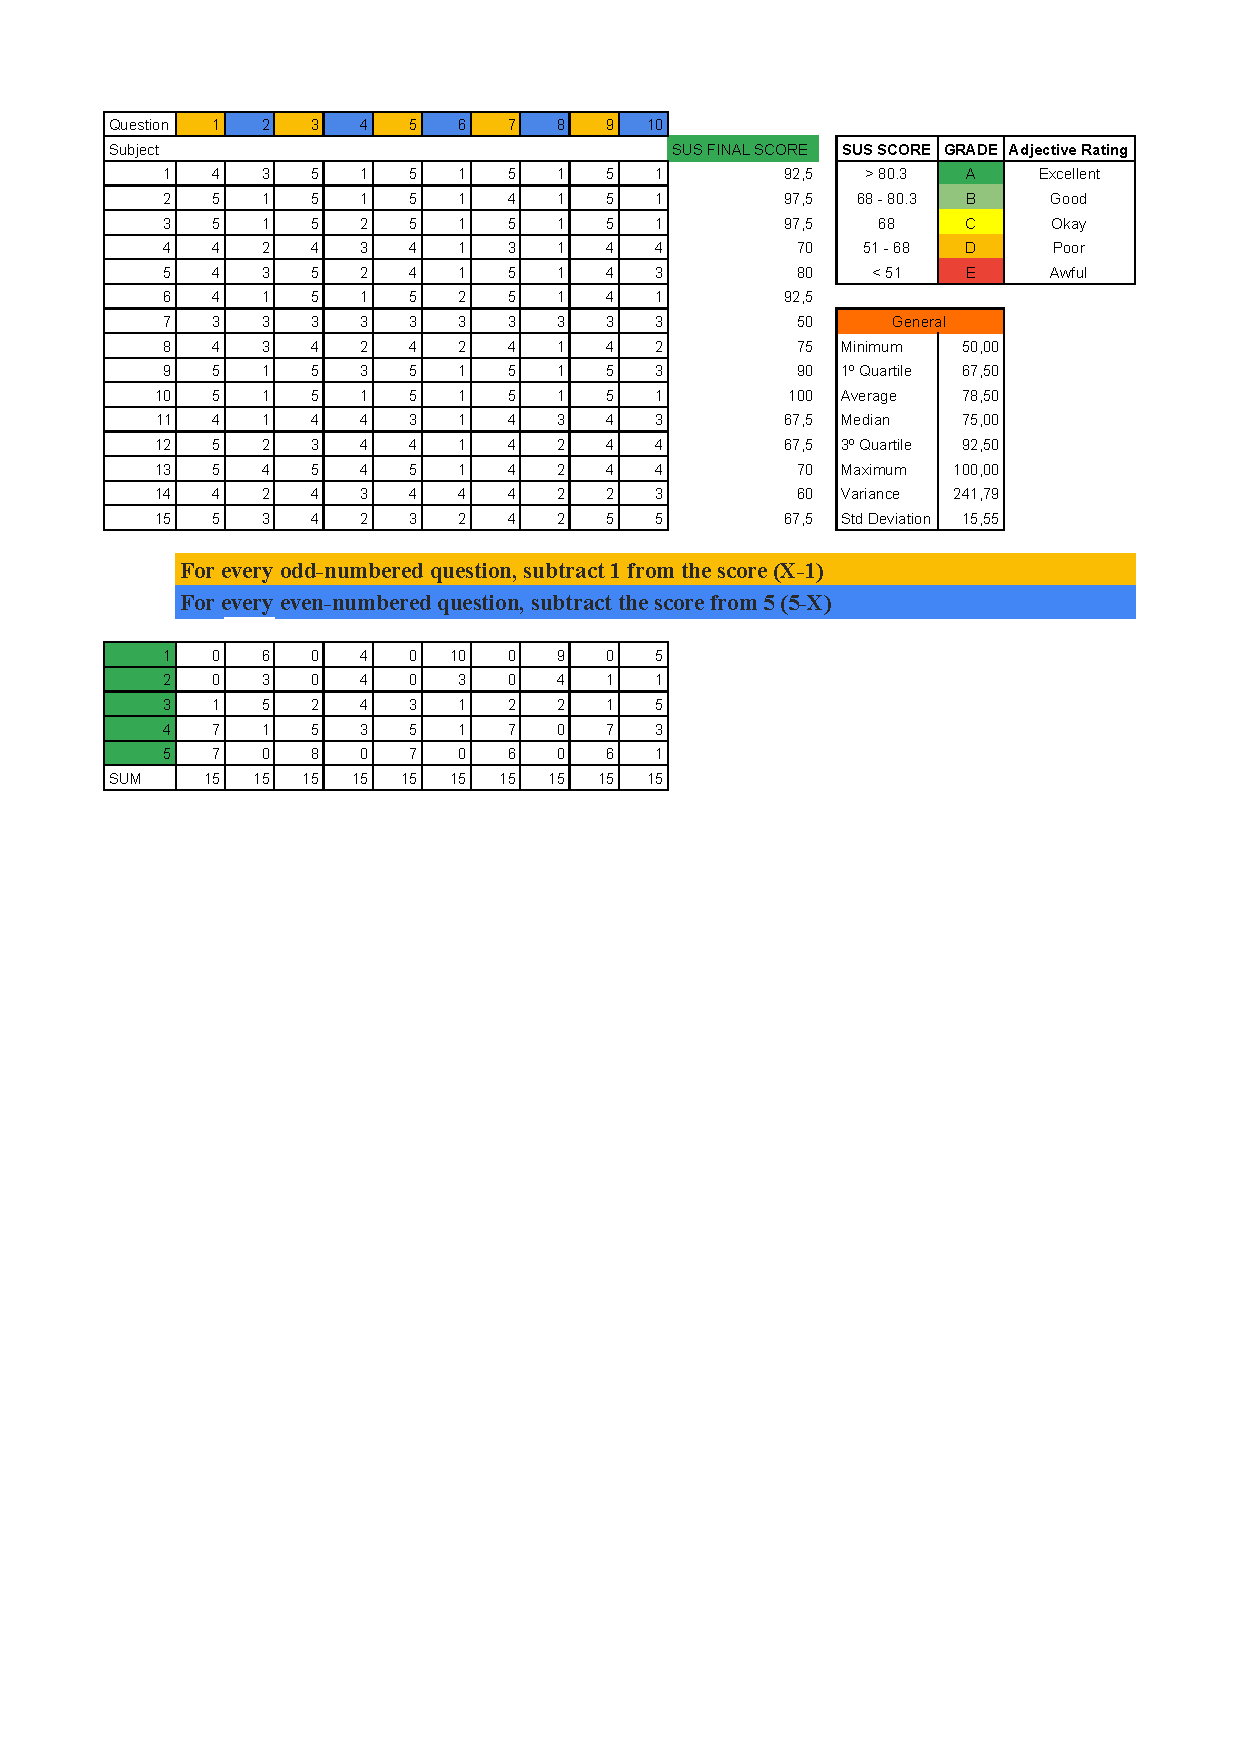
\includepdf[pages=-, frame=false, scale=0.80]{postextuais/appendix/EX3-SUS-ERtext.pdf}
    % \caption{EX3 - SUS - ERtext.}
    \label{fig:ex3EmocardsERtext}
\end{figure}

\end{apendicesenv}

% ==============================================================================
\chapter{Reference models and examples}\label{ap:referenceModels}
% ==============================================================================


\section{Instrument 1 (portuguese description)} \label{ap:Inst1Exp}

    \begin{figure}[!htb]
        \centering
        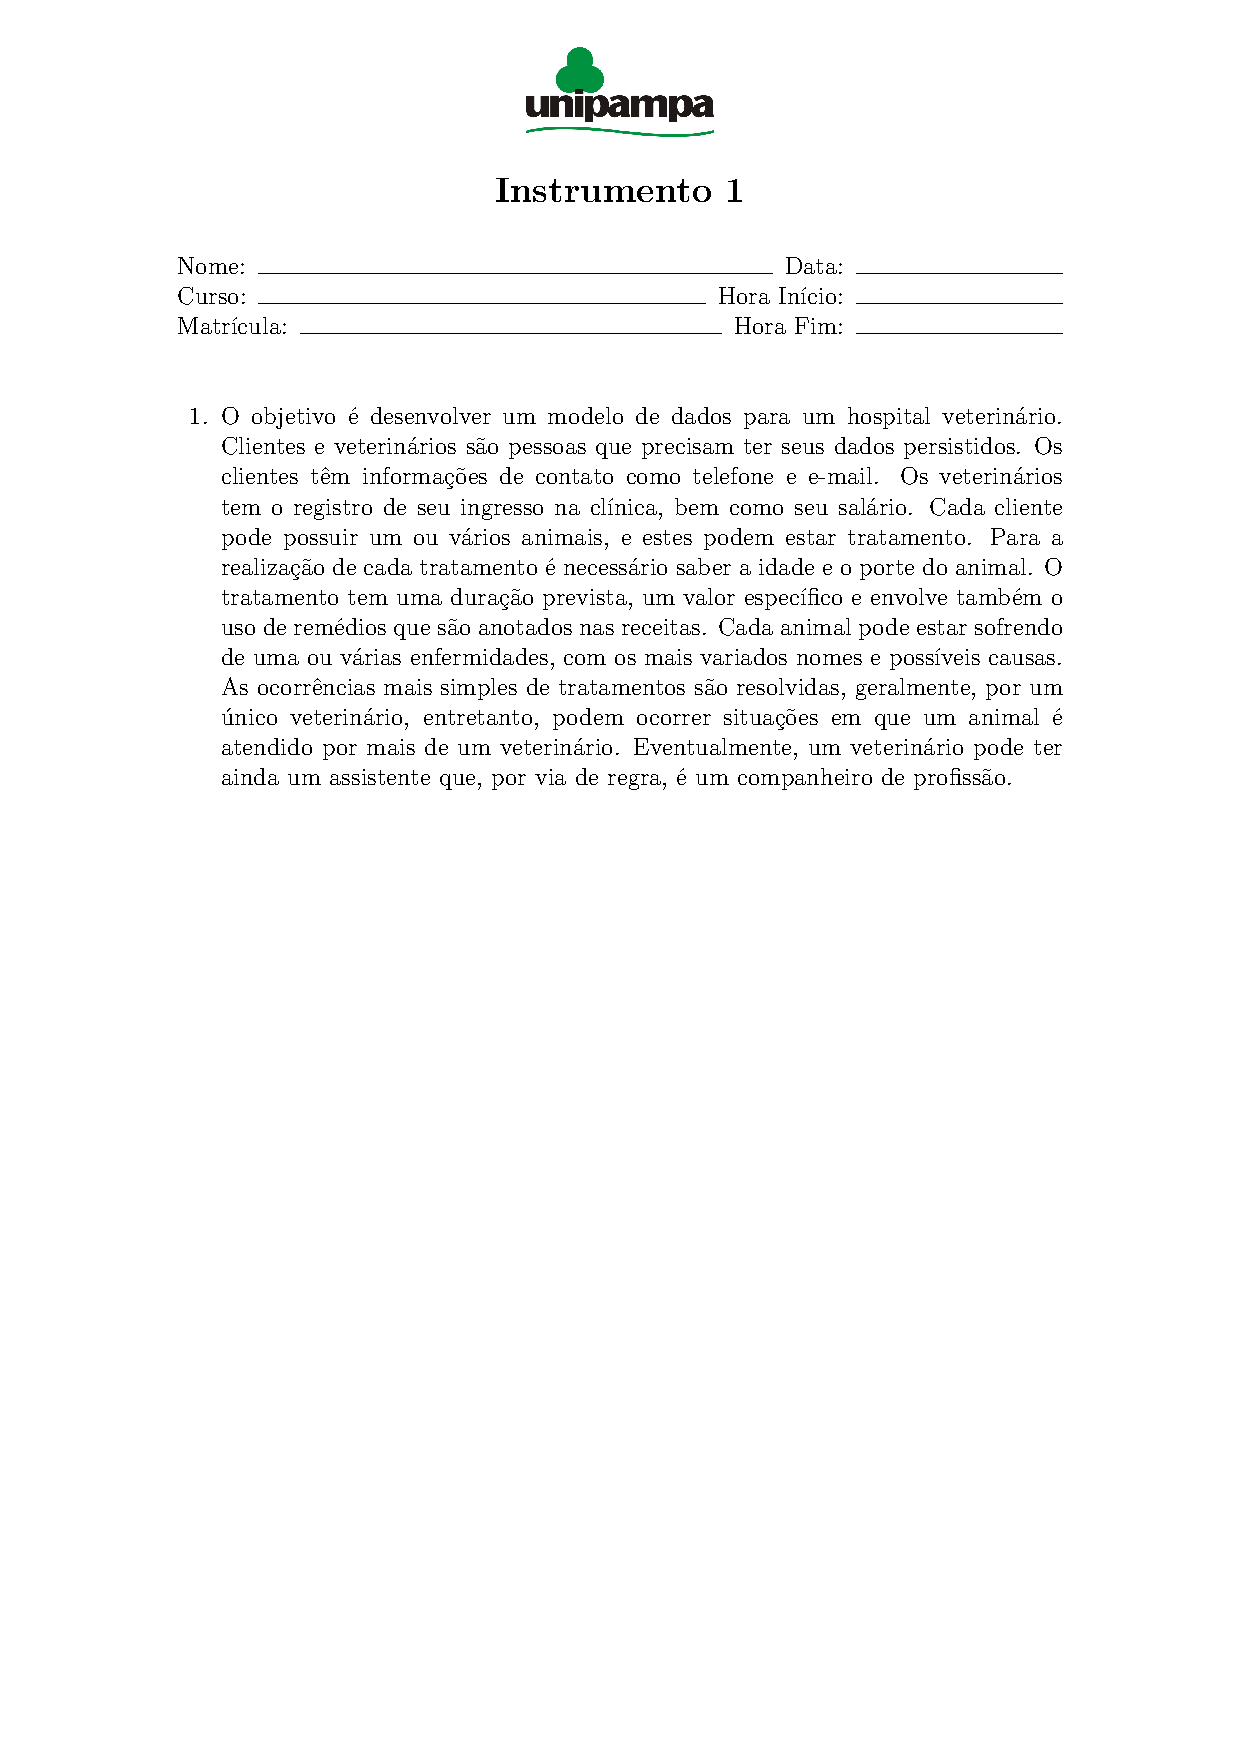
\includepdf[pages=-, frame=true, scale=0.65]{postextuais/appendix/Instrumento1.pdf} 
    \end{figure}

\newpage

\section{Instrument 2 (portuguese description)} \label{ap:Inst2Exp}

    \begin{figure}[!htb]
        \centering
        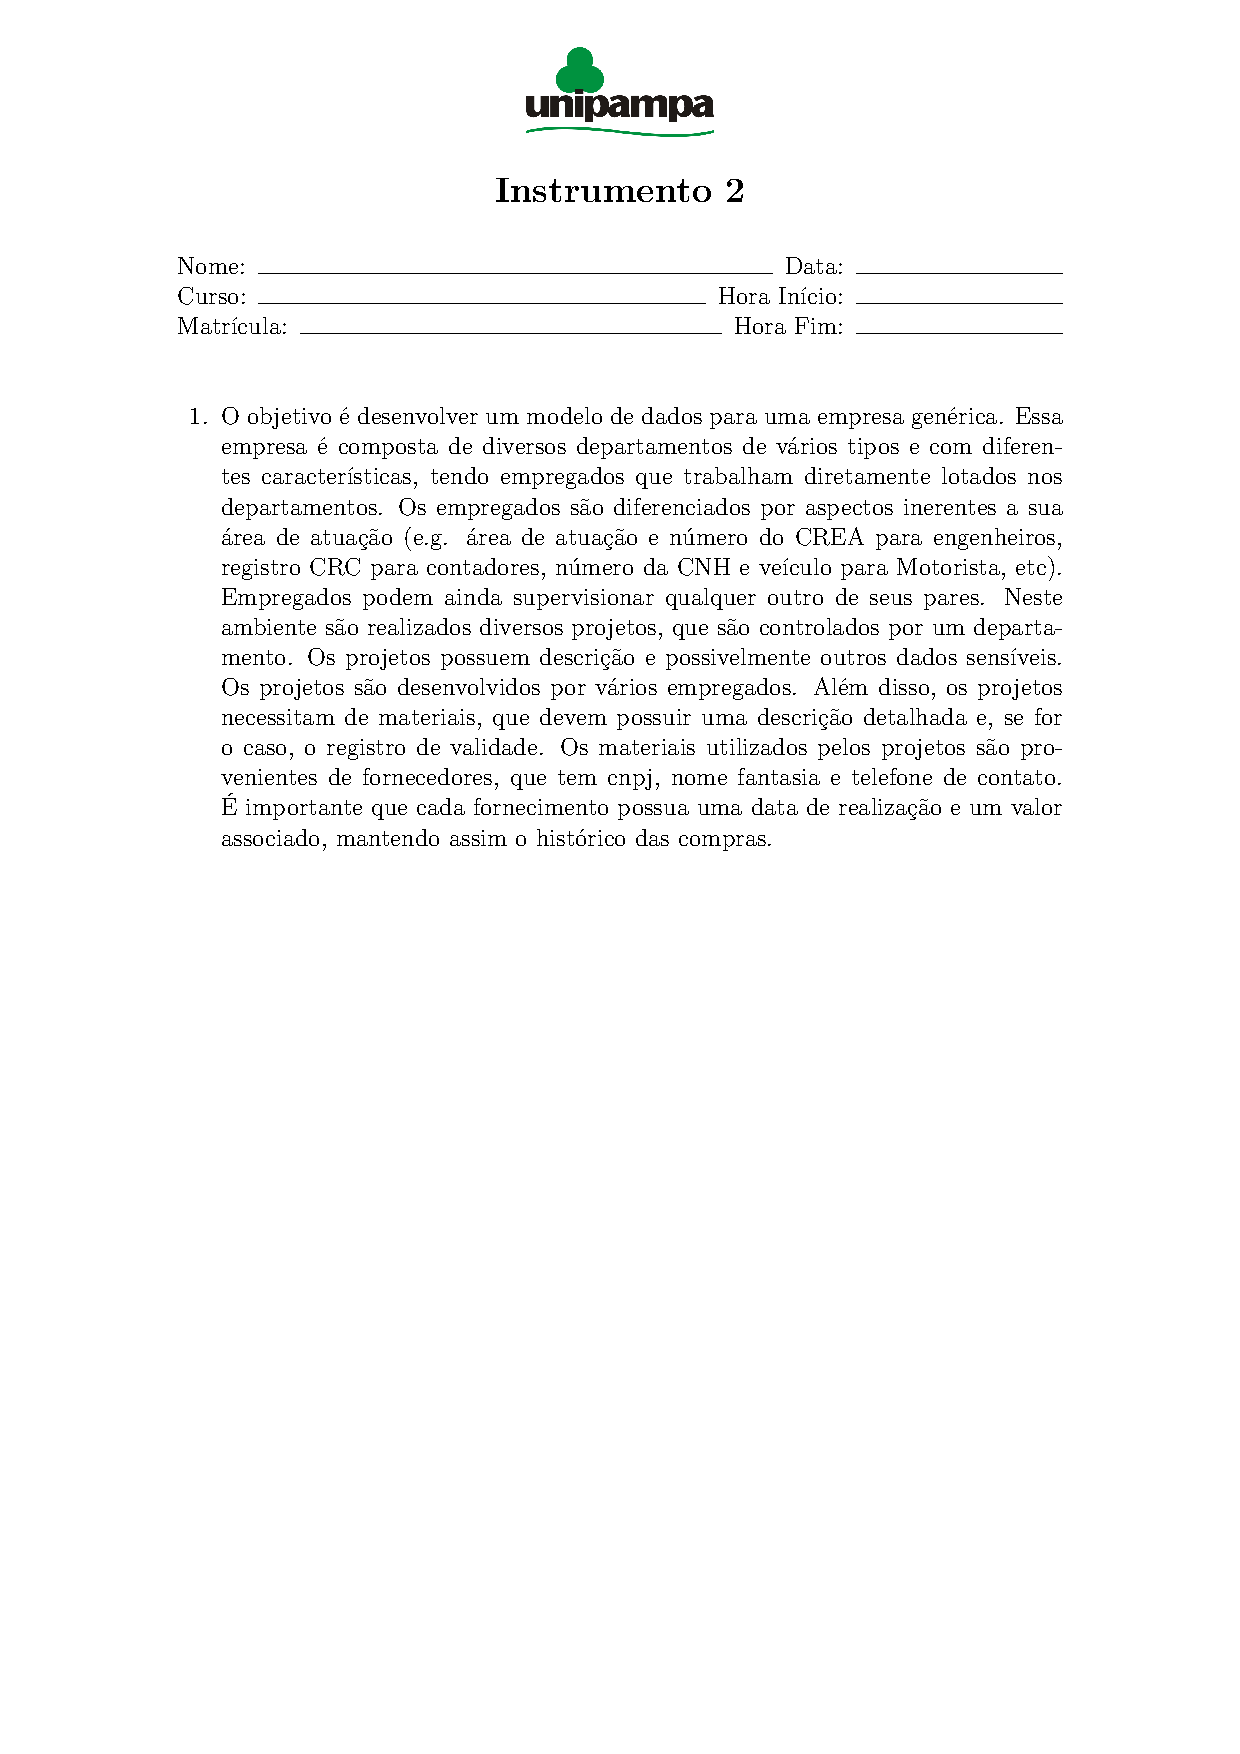
\includepdf[pages=-, frame=true, scale=0.65]{postextuais/appendix/Instrumento2.pdf} 
    \end{figure}

\newpage

\section{Reference model - brModelo (Instrument 1)}

\begin{figure}[!htb]
    \centering
    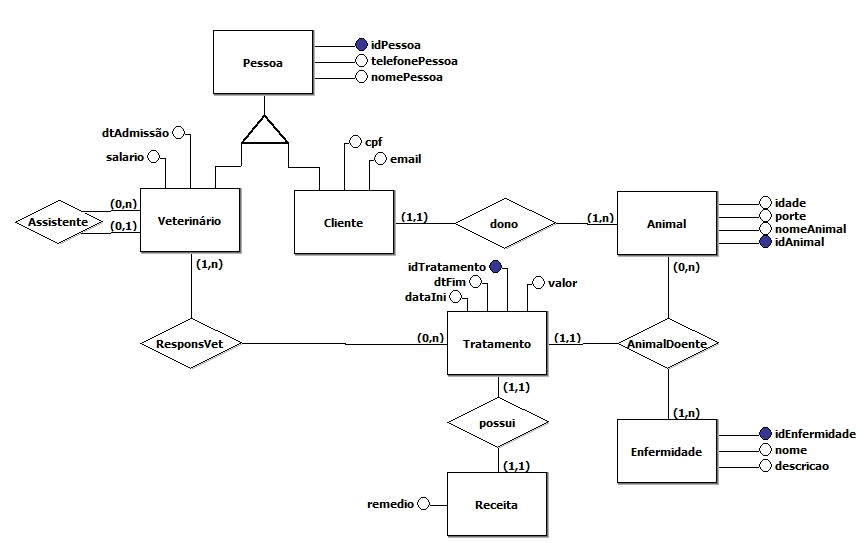
\includegraphics[scale=0.5]{postextuais/Instrument1 (brModelo Reference Model).jpg}
    % \caption{Caption}
    \label{fig:referenceModelbrModeloInst1}
\end{figure}

\newpage

\section{Reference model - brModelo (Instrument 2)}

\begin{figure}[!htb]
    \centering
    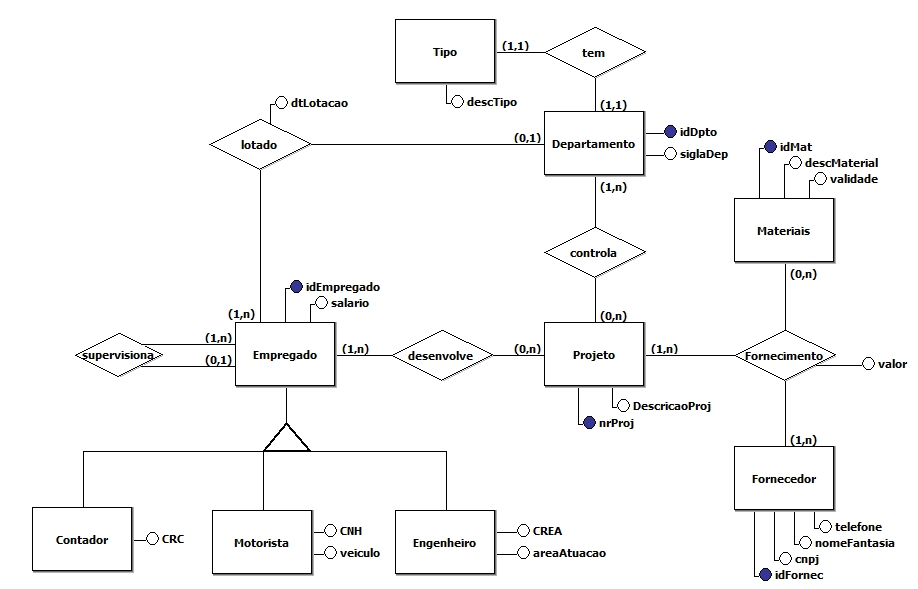
\includegraphics[scale=0.5]{postextuais/Instrument2 (brModelo Reference Model).jpg}
    % \caption{Caption}
    \label{fig:referenceModelbrModeloInst2}
\end{figure}

\newpage

\section{Reference model - ERtext (Instrument 1)}

\begin{figure}[!htb]
    \centering
    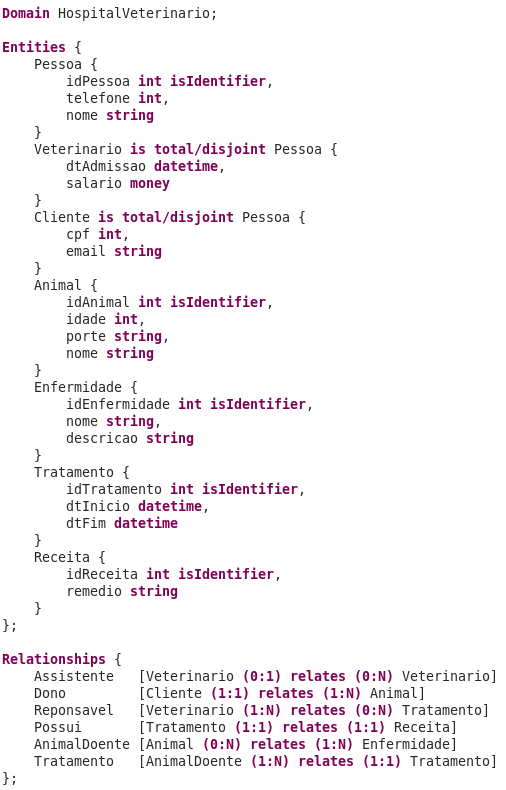
\includegraphics[scale=0.5]{postextuais/appendix/Instrument1-ReferenceModel-ERtext.png}
    % \caption{Caption}
    \label{fig:referenceModelERtextInst1}
\end{figure}

\newpage

\section{Reference model - ERtext (Instrument 2)}

\begin{figure}[!htb]
    \centering
    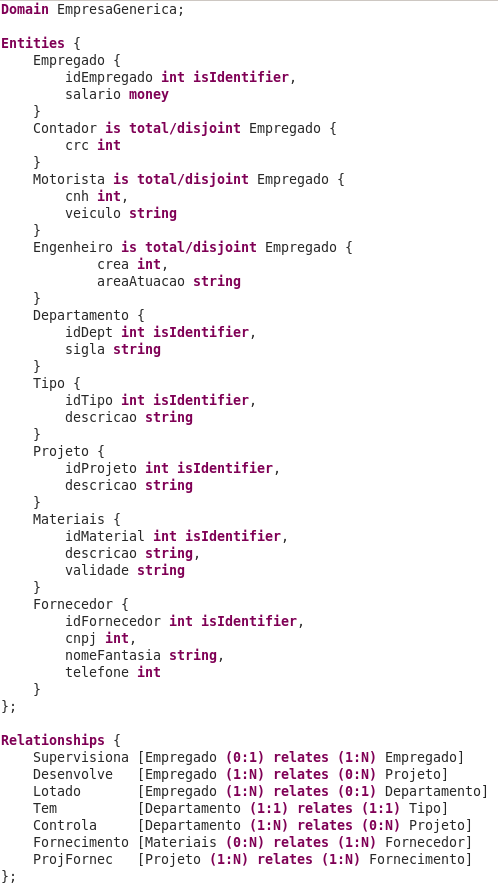
\includegraphics[scale=0.5]{postextuais/appendix/Instrument2-ReferenceModel-ERtext.png}
    % \caption{Caption}
    \label{fig:referenceModelERtextInst2}
\end{figure}

\newpage

\section{Modeled examples by a subject - brModelo}

\begin{figure}[!htb]
    \centering
    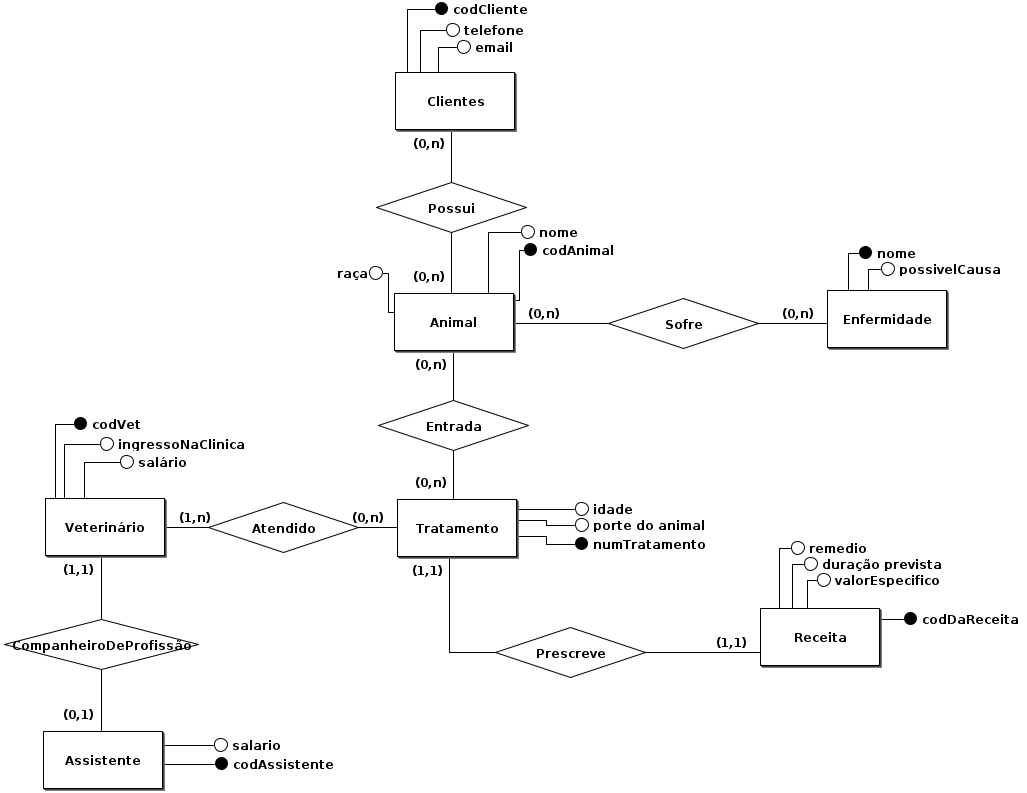
\includegraphics[scale=0.4]{postextuais/appendix/ExampleSubject-brModelo.png}
    % \caption{Caption}
    \label{fig:my_label}
\end{figure}

\newpage

\section{Modeled examples by a subject - ERtext}

\begin{figure}[!htb]
    \centering
    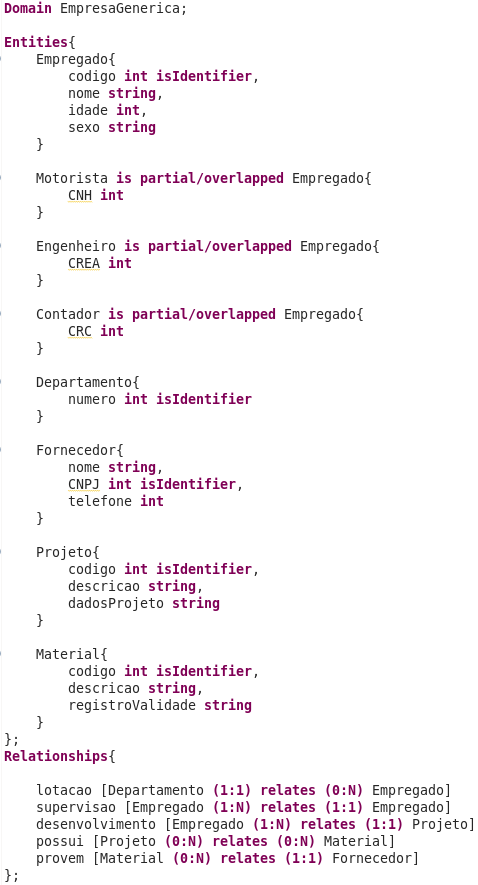
\includegraphics[scale=0.5]{postextuais/appendix/ExampleSubject-ERtext.png}
    % \caption{Caption}
    \label{fig:my_label}
\end{figure}